\documentclass{article}
\usepackage[a4paper, margin=2.8cm]{geometry}
\usepackage{graphicx} % Required for inserting images
\usepackage{amssymb}
\usepackage{amsmath}
\usepackage{amsthm}
\usepackage{physics}
\usepackage{hyperref}
\usepackage{bbm}
\usepackage{cleveref}
\usepackage{thmtools}
\usepackage{pdfpages}
\usepackage{todonotes}

\newcommand{\add}[1]
{\todo[inline,color=green,caption={}]{#1}}
\newcommand{\remark}[1]{\todo[inline,color=orange,caption={}]{#1}}
\newcommand{\adrian}[1]{\todo[inline,color=red,caption={}]{#1}}
\newcommand{\XX}{{\color{red}{XXX}}}

\newtheorem{definition}{Definition}
\newtheorem{theorem}{Theorem}[section]
\newtheorem{corollary}{Corollary}[theorem]
\newtheorem{lemma}[theorem]{Lemma}
\newtheorem{proposition}[theorem]{Proposition}
\newtheorem{condition}{Condition}
\newtheorem{conjecture}[theorem]{Conjecture}

\title{Low dimensional counterexamples to the weighted hot spots conjecture}
\author{Adrian Wüthrich}
\date{May 2025}

\setlength{\parindent}{0pt}

\begin{document}

\newcommand{\R}{\mathbb{R}}
\newcommand{\E}{\mathbb{E}}
\newcommand{\inner}[2]{\langle #1, #2 \rangle}

%%% =================== NUMERICAL VALUES ===================

\newcommand{\dimension}{10^{12}}
\newcommand{\eiglowerdelta}{0.03}
\newcommand{\tzero}{50}
\newcommand{\normphizero}{2.5}

%%% ========================================================


\maketitle

\begin{abstract}
    Recently \cite{pont_convex_2024} found counterexamples to the Hot Spots conjecture in sufficiently high dimensions. While the dimension at which the conjecture starts to be false is in principle effective, the number arising from a direct interpretation of the proof is excessively large.  This work initiates a program towards finding low-dimensional counterexamples to the Hot Spots conjecture, by focusing on a related 'weighted' version of the conjecture, which served as a key surrogate problem in the original disproof. By constructing a specific family of convex domains and potentials, we establish an effective lower bound, showing that for dimensions $d \ge \dimension$, counterexamples to the weighted Hot Spots conjecture exist.
\end{abstract}


\section{Introduction}

Let $\Omega$ be a bounded, connected, regular enough domain in $\mathbb R^d$. Let $u(x,t)$ be the solution in $\Omega$ of the heat equation in $\Omega$ with insulating boundary conditions (Neumann) and initial temperature $u(x,0)=u_0(x)$. That is,

\begin{equation}
    \begin{cases}
        \partial_t u(x,t) = \Delta u(x,t) & \text{ for } (x,t)\in \Omega^\circ\times \mathbb R_{>0}\\
        \partial_n u(x,t) = 0 &\text{ for } (x,t)\in \partial \Omega \times \mathbb R_{>0} \\
        u(x,0) = u_0
    \end{cases}
\end{equation}

Under mild regularity conditions in $\Omega$, the temperature $u(x,t)$ of the domain converges uniformly to the average temperature of the domain as $t$ goes to infinity. In other words, the functions $u_t:= u(t,\cdot)$ converge, as $t\to \infty$, to the constant function with value $\overline u:= \frac 1 {|\Omega|}\int_\Omega u_0(x) dx$ in the in $L^\infty(\Omega)$ sense.

Rauch's Hot Spots conjecture aims to understand the largest fluctuations of $u_t$, namely, the points where $u_t$ attains its maximum and minimum. It asserts that the global maxima and minima of $u_t$ (the hottest and coldest points in $\Omega$ for large times) approach the boundary of $\Omega$.  In order to understand this asymptotic behavior of $u_t$ for large times, one can use the method of separation of variables. 

The Neumann-Laplace operator $-\Delta$ in $\Omega$ is a self-adjoint operator with discrete eigenvalues $0= \lambda_0<\lambda_1 \le\lambda_2\le \lambda_3 \dots$ with an associated orthonormal eigenbasis $\phi_0, \dots, \phi_k\dots$ satisfying 
\begin{equation}
    \begin{cases}
        -\Delta \phi_i = \lambda_i \phi_i \text{ in } \Omega^\circ \\
        \partial_n \phi_i = 0 \text{ in }\partial \Omega
    \end{cases},
\end{equation}
with $\phi_0\equiv \frac{1}{|\Omega|^{1/2}}$ a constant function. The method of separation of variables then gives us a solution to the heat equation $$u_t(x) = \sum_{k \ge 0} \inner{u_0}{\phi_k}\phi_k e^{-\lambda_k t}.$$


This shows, in particular, that the heat distribution converges to the mean \( \int_\Omega u_0 \) as \( t \to \infty \), at least in the $L^2(\Omega)$ sense. The convergence in $L^\infty(\Omega)$ follows once one shows, under mild regularity conditions on $\Omega$, that the functions $u_t(x)$ are Hölder-continuous. 

Let $k_0>0$ be the first non-zero index $k$ such that $\langle u_0, \phi_k\rangle \neq 0$, and assume, for simplicity, that $\lambda_{k_0+1}>\lambda_{k_0}$.The function $\tilde u_t(x,t) := e^{\lambda_{k_0} t}(u(x,t)-\bar u)$ has maxima and minima in the same locations as $u_t$, and
$$
\tilde u_t = 
\langle u_0, \phi_{k_0}\rangle \phi_{k_0}
+
\sum_{n\ge 1}e^{-(\lambda_{k_0+n}-\lambda_{k_0})t}
\langle u_0, \phi_{k_0+n}\rangle \phi_{k_0+n}.
$$
As $t\to \infty$, the functions $\tilde u_t$ must then converge exponentially fast to the function $\langle u_0, \phi_{k_0}\rangle \phi_{k_0}$, and in particular, 

\begin{lemma}
    Under sufficient regularity for $\Omega$, the functions $\tilde u_t$ converge uniformly to a nonzero multiple of $\phi_{k_0}$. In particular, the extremal points of $\tilde u_t$ and of $u_t$ converge subsequentially to extremal points of $\phi_{k_0}$.
\end{lemma}

\begin{figure}[h]
  \centering
  \includegraphics[width=0.2\textwidth]{figures/Archive 2/static_ball_1.png}
  \includegraphics[width=0.2\textwidth]{figures/Archive 2/static_ball_2.png}
  \includegraphics[width=0.2\textwidth]{figures/Archive 2/static_ball_3.png}
  \includegraphics[width=0.2\textwidth]{figures/Archive 2/static_ball_4.png}
  \caption{From left to right: The first four Laplacian eigenfunctions $\phi_1,\phi_2,\phi_3,\phi_4$ on a Disk.}
  \label{fig:modes}
\end{figure}

It is relatively straightforward to find examples of initial conditions for which not all extrema converge to the boundary. Consider the first four Neumann eigenfunctions of the Laplacian on a disk, as illustrated in \Cref{fig:modes}. By selecting $u_0$ such that $\inner{u_0}{\phi_1} = \inner{u_0}{\phi_2} = \inner{u_0}{\phi_3} = 0$ and $\inner{u_0}{\phi_4} = 1$, the extremal points of $\tilde u_t$ converge to the extremal points of $\phi_4$, which do not entirely lie on the boundary. However, this straightforward counterexample can be dismissed by setting constraints on the initial condition; for \emph{generic} initial conditions $u_0$, all coefficients $\langle u_0, \phi_k\rangle$ are nonzero, and $k_0 = 1$. This leads to the Hot Spots conjecture, as commonly referenced in the literature:

\begin{conjecture}[\cite{rauch_lecture_1975}]
    For \emph{nice enough} bounded domains $\Omega\subset \mathbb R^d$, the global extrema of $\phi_1$ are attained in $\partial \Omega$.
\end{conjecture}
 
The definition of \emph{nice} is deliberately vague at this point, and it remains a challenge to find natural classes of domains for which the conjecture is true. A significant challenge of the conjecture is that Laplace eigenfunctions can only be explicitly computed for very limited domains, like balls, triangles, and squares. For more interesting classes of domains, identifying where the first eigenfunction reaches its maximum remains open. Potential classes of \emph{nice} domains that have been considered include domains with a smooth boundary (disproven by a counterexample with a planar domain with two holes \cite{burdzy_counterexample_1999}), simply connected domains in $\mathbb R^2$ (currently open), and convex domains in $\mathbb R^d$ (disproven in high enough dimensions \cite{pont_convex_2024}).

This work focuses on understanding this late scenario. While the argument in \cite{pont_convex_2024} can technically be made effective, the dimensions one would obtain by a naive tracking of the constants would be extremely large\footnote{A naive implementation of \cite{pont_convex_2024} would provide a bound $e^{e^{C}}$ for some constant $C$ that could in principle be optimized, but most likely not below $~20$. This would give, in the most optimistic case, $d_0\ge 10^{10^4}$.} The goal of this work is to improve on these types of estimates.

\paragraph{What happens when there are multiple ground eigenfunctions?}

The eigenspace of the eigenvalue $\lambda_1$ is not necessarily one-dimensional. This is the case, for example, for both the square and the ball. In this case, one could make multiple versions of the Hot Spots conjecture, namely whether it holds \emph{for any}, or \emph{for some} eigenfunction in the first eigenspace. More precisely, Bañuelos-Burdzy \cite{banuelos_hot_1999} introduced three small variations of the Hot Spots conjecture, namely
\begin{enumerate}
    \item[(HS1)] For every eigenfunction $\varphi_{1}(x)$ corresponding to $\lambda_1$ which is not identically $0$, and all $y \in D$, we have 
\[
\inf_{x \in \partial D} \varphi_{1}(x) < \varphi_{1}(y) < \sup_{x \in \partial D} \varphi_{1}(x).
\]

\item[(HS2)] For every eigenfunction $\varphi_{1}(x)$ corresponding to $\lambda_1$ and all $y \in D$, we have 
\[
\inf_{x \in \partial D} \varphi_{1}(x) \leq \varphi_{1}(y) \leq \sup_{x \in \partial D} \varphi_{1}(x).
\]

\item[(HS3)] There exists an eigenfunction $\varphi_{1}(x)$ corresponding to $\lambda_1$ which is not identically $0$, and such that for all $y \in D$, we have 
\[
\inf_{x \in \partial D} \varphi_{1}(x) \leq \varphi_{1}(y) \leq \sup_{x \in \partial D} \varphi_{2}(x).
\]
\end{enumerate}

All constructions of this work will have a simple first eigenspace with a maximum on the interior. This will allow us to talk about \emph{the} first eigenfunction, and disprove the three versions at once.

\subsection{The first Laplace eigenfunction and the Poincaré-Sobolev constant} \label{soincare_popolev}

The main feature that separates the first Laplace eigenfunction from higher Laplace eigenfunctions is that it is the minimizing function of the Poincaré inequality.
We define the Poincaré constant $C_p (\Omega)$ of a set $\Omega$ as the smallest constant such that the inequality
$$
\int_{\Omega}|f-\overline f|^2 dx \le C_p(\Omega) \int_{\Omega} |\nabla f|^2 dx.
$$

The essential point to note is that this constant is, in fact, equal to $1/\lambda_1(\Omega)$, and this equality is achieved only for the Neumann Laplace eigenfunctions associated with the eigenvalue $\lambda_1$. To observe this at a formal level (i.e., disregarding the theory of existence of minimizers that satisfy the Poincaré inequality, e.g. see \cite{evans_partial_1998}), one can analyze the critical points of the functional
$$
E(f):=\frac{\int_{\Omega} |\nabla f|^2 \, dx}{\int_{\Omega}|f-\overline f|^2 \, dx}.
$$
Critical points are points for which the first variation is zero, that is, points that satisfy
$$
\left.\frac{d}{dt}\right|_{t=0} E(f+tg) = 0
$$
for any $g\in C^{\infty}(\overline \Omega)$. The critical points of $E$ are exactly the Neumann eigenfunctions of the Laplacian. To see that, assume (without loss of generality by scaling invariance) that $\int_{\Omega} (f - \overline f)^2 dx =1$. In this case, one can compute
$$
\left. \frac{d}{dt} \right|_{t=0}E(f+t\varphi)
=
2\int_{\Omega} \nabla f \cdot \nabla \varphi dx
-2 \lambda_f
\int_{\Omega} (f-\overline f) \varphi dx,
$$
where $\lambda_{f}:= \int |\nabla f|^2 dx$. By setting the right-hand side to zero and integrating by parts, we obtain
\begin{equation} \label{eq:poincare_int_by_parts}
\lambda_f\int_{\Omega} (f-\overline f) \varphi dx
+ \int_\Omega (\Delta f) \varphi \dd{x} = \int_{\partial \Omega} (\nabla f \cdot n) \varphi \dd{x}.
\end{equation}
In particular, for all functions $g$ that vanish on $\partial \Omega$ we have
$$
\int_{\Omega} (\lambda_f(f-\overline f) + \Delta f) g \dd{x} = 0.
$$
By the fundamental lemma of variational calculus this shows that $\lambda_f(f-\overline f) + \Delta f = 0$, i.e. $f-\overline f$ is an eigenfunction of $-\Delta$ to the eigenvalue $\lambda_f$. Plugging this back into \Cref{eq:poincare_int_by_parts}, it follows immediately that for any function $h \in C^\infty(\overline{\Omega})$ we have
$$
\int_{\partial \Omega} (\nabla  f \cdot n) h \dd{x} = 0
$$
and therefore $\nabla f \cdot n = 0$. Notice how we obtained the Neumann boundary condition on $f$ without apriori assuming it.

Restricting to functions with zero mean we obtain the well known Rayleigh quotient characterization of eigenvalues.

\subsection{Weighted hot spots conjecture}

A key step in disproving the Hot Spots conjecture for high-dimensional convex sets is finding counterexamples to a stronger (weighted) version of the conjecture. The weighted hot spots conjecture asserts that there exists a convex potential \( V \) defined on a convex domain \( \Omega \) such that the first Neumann eigenfunction of the operator \( \mathcal{L} := -\Delta + \nabla V \cdot \nabla \) attains its maximum on the boundary of \( \Omega \). The operator $L$, similarly to $-\Delta$, has a variational characterization.


\subsubsection*{Variational interpretation of the weighted hot spots conjecture}

In \Cref{soincare_popolev} we established that the Neumann eigenfunctions minimize the Rayleigh quotient over all zero mean functions. For the Neumann eigenfunctions of $-\Delta + \nabla V \cdot \nabla$ we have an analogous characterization, albeit with respect to a measure weighted by $e^{-V}$.

\begin{proposition} \label{prop:var_char}
The first non-trivial Neumann eigenvalue of the operator $\mathcal{L} = -\Delta + \nabla V \cdot \nabla$ is given by
\[
    \lambda^{(1)}_{\Omega, V} = \min_{\substack{f \in C^2(\Omega) \\ \int_\Omega f e^{-V} \dd{x} = 0}} \frac{\int_\Omega |\nabla f|^2 e^{-V} \dd{x}}{\int_\Omega |f|^2 e^{-V} \dd{x}},
\]
and this minimum is attained exactly by the eigenfunction $\phi_1$ corresponding to \( \lambda^{(1)}_{\Omega, V} \).
\end{proposition}
\begin{proof}
The proof is analogous to the one for the Laplacian. The key equality, analogous to \Cref{eq:poincare_int_by_parts} is the following integration by parts:
$$
\int_{\Omega} \nabla \phi \nabla \psi e^{-V(x)} dx = \int_{\partial \Omega} \phi \nabla \psi \cdot n \, e^{-V(x)} dx + \int_{\Omega} \phi (-\Delta \psi + \nabla V \cdot \nabla \psi) e^{-V(x)} dx.
$$
The rest of the proof is verbatim.
\end{proof}


\subsubsection*{The $L$ as a Laplace operator on thin domains}


This version of the hot spots conjecture can be viewed as a hot spots conjecture for thin plates with a cross-sectional volume of \( e^{-V} \). Suppose the domain $\Omega$ is of in the form of $P \times T$, where $T$ is very thin in all directions. On such a domain, any regular enough function is practically constant in the thin direction. The first Neumann eigenfunction achieves the minimum for $\inner{f}{\Delta f}_{L^2}$ over normalized functions. Observe that $\inner{f}{\Delta f}_{L^2} = -\int_{P \times T} |\nabla f|^2 \dd{x} \dd{y}$, but since $f$ is nearly constant in the thin direction, it follows that $|\nabla f|^2 \approx |\nabla_{P} f|^2 \dd{x}$. Consequently, integration over $T$ contributes a multiplicative factor of $e^{-V}$, thus $\inner{f}{\Delta f}_{L^2} \approx -\int_{P} |\nabla f|^2 e^{-V} \dd{x}$. Through integration by parts, the expression on the right becomes $\inner{f}{\mathcal{L} f}_{L^2(e^{-V})}$. We will show that the functions which minimize $\inner{f}{\mathcal{L} f}_{L^2(e^{-V})}$ are indeed Neumann eigenfunctions of the operator $\mathcal{L}$. This heuristic illustrates how the weighted hot spots conjecture aligns with the properties of the first Neumann eigenfunction for the operator $\mathcal{L}$, considering the measure is weighted by $e^{-V}$.

The idea of using extra dimensions to simulate a new effective PDE is at the heart of the counterexample in \cite{pont_convex_2024}. A key step is to disprove the weighted version of the conjecture. In this work, we aim to find an effective upper bound on the dimension after which the weighted hot spots conjecture fails.

\subsection{The main result}

By constructing a family of convex potentials that depend on the dimension, we establish an explicit lower bound on the dimension for which the weighted hot spots conjecture is false. Our main result is as follows:

\begin{theorem}
There exists a convex potential $V$ on a convex domain $\Omega \subset \R^d$ for $d \ge \dimension$ such that the first Neumann eigenfunction $\phi$ attains its maximum in the interior of $\Omega$.
\end{theorem}

\subsubsection*{Acknowledgements}
The author expresses his sincere gratitude to his supervisor, Dr. Jaume De Dios, for his invaluable guidance and support. The proof strategy originated from him, as did the figures in the Introduction. He also contributed the proof of \Cref{lem:coupling}. I am deeply grateful for his help editing and reviewing this work.

\section{Strategy and outline of the proof}

This section lays out the proof strategy and how the main estimates interact. The sequence of domains $\Omega_d$ will be of the form $[-M,M]\times B_R(\mathbb R^d)$ (for $M,R$ chosen later through the proof), with potentials that are radial in the second coordinate.

Our aim is to reduce this $d+1$-dimensional problem to an effective two-dimensional setting, construct a tractable approximation to the first Neumann eigenfunction, and obtain pointwise estimates that contradict the hot spots property. The argument proceeds in five steps; precise statements and details appear in the subsections that follow.

\begin{enumerate}
    \item \textbf{Cylindrical Domains and Coordinates:} We exploit the radial symmetry of our chosen domains to show that the first Laplace eigenfunction of $(\Omega_d, V_d)$ must also be radial. This allows us to reduce the high dimensional problem to an effective two-dimensional problem on a rectangular domain with an effective potential of the form \( V_d(x,w)=(d-1)(V_0(x,|w|)-\log |w|) \). In this domain, the Neumann eigenfunction of \( -\Delta + \nabla V_d \cdot \nabla \) attains its maximum in the interior.

    \item \textbf{$L^2$ convergence of the effective problem:} In the effective two-dimensional setting we $L^2$-normalize the first Neumann eigenfunctions $\phi_d$ with respect to the probability measures $\frac{1}{Z_d}e^{-V_d} dx$. This immediately shows that $\phi_d$ must achieve a value of at least $1$ at some point within the interior. Consequently, our objective shifts to showing that $\phi_d$ is less than $1$ on the boundary. We construct $V$ such that as $d \to \infty$, the measure $\frac{1}{Z_d}e^{-V_d}$ converges to the uniform measure on a one-dimensional line segment. Then we would expect that the eigenfunctions converge to the ones of the one-dimensional Laplacian on the said segment. The eigenfunction in one dimension serves as a guide to identify an auxiliary function $f_0$, which has the property that $\|\phi_d-f_0\|_{L^2(Z_d^{-1}e^{-V_d}dx)}$ converges to zero as $d \to +\infty$. 

    \item \textbf{$L^\infty$ estimates via ultracontractivity:} An average ($L^2$) approximation is insufficient to control the maximum of the eigenfunction. We must upgrade our $L^2$ estimate to a pointwise ($L^\infty$) one. This is achieved by considering the function $\tilde \phi_d = e^{\lambda t} P_t f_0$ for some $t>0$, $f_0 \in L^2$ where $P_t$ is the semigroup associated with $-\Delta + \nabla V \cdot \nabla$. This construction allows us to invoke powerful estimates on semigroups, known as ultracontractivity estimates.
    
    \item \textbf{Boundary estimates through probabilistic interpretation:} We use a probabilistic interpretation of the semigroup $(P_t)_{t \ge 0}$, viewing it as the expectation of a function along the paths of a diffusion process. For large $d$, this diffusion is dominated by a deterministic drift, which corresponds to the gradient flow $\Phi_t$ of the potential. We show that for $d$ being sufficiently large, $\tilde \phi_d(x) \approx f_0(\Phi_t(x))$. Given that $V$ is convex, we have good control over the flow lines, thereby establishing that for any point $x$ on the boundary, $f_0(\Phi_t(x))$ is small.

    \item \textbf{Synthesis of Estimates:} Finally, we combine the above results. The $L^2$ normalization implies the eigenfunction must be large somewhere in the domain. Our boundary estimates show that the approximating function $\tilde \phi$ is small on the boundary. Since our approximation error in $L^\infty$ scales as $d^{-1/4}$, we can pass the boundary estimate to the true eigenfunction for $d$ large enough.
\end{enumerate}

\subsection{Cylindrical Domains and Coordinates}


\subsubsection*{The effective problem in cylindrical coordinates} 
We will consider cylindrical domains of the form $[-100,100]\times B_{10}(\mathbb R^d)$ with a radial potential $V_d(x,y):= (d-1)V_0(x,|y|)$, and show that, under reasonable properties for $V_0$, for $d$ large enough the first Neumann Laplace eigenfunction will be radial. Indeed, we will show:

\begin{restatable}{proposition}{propradial}
    Let $\Omega:=[-M,M]\times B_{10}(\mathbb R^d)$, and $V: \Omega \to \mathbb R$ be a radial potential. Then if $\lambda^{1}_{\Omega,V}<\frac{d}{100}$, the first eigenfunction $\phi_{\Omega,V}$ is radial in the second coordinate.
\end{restatable}
    


In our case, $R=10$, and $\lambda^{1}_{V_d} \le 1+10^{-14}$ for $d \ge 400$, see \Cref{prop:eig_upper_bound}. Once we know that the first eigenfunction is radial, it must be the minimizer of 
$$
\frac{\int_{-M}^M \int_0^R |\nabla f(x, r)|^2 r^{d-1} e^{-(d-1) V(x,r)} dx dr}{\int_{-M}^M \int_0^R |f(x, r)|^2 r^{d-1} e^{-(d-1) V_0(x,r)} dx dr}.
$$
We can write $r^{d-1} e^{-(d-1) V_0(x,r)}$ as $e^{-(d-1)(V_0(x,r)-\log(r))}$. Therefore, this minimization problem is the Rayleigh quotient with effective potential $V^{eff}_d (x,r) := (d-1)(V_0(x,r)-\log(r))$. In particular, by \Cref{prop:var_char}, $\psi_d(x,y) = \phi_d(x,|y|)$ is the first Neumann eigenfunction of $L_{V^{eff}_d}$. We have reduced the problem to a domain of the form $[-M,M]\times [0,R]$ with a convex potential of the form $V_d(x,y) = (d-1)(V_0(x,y)-\log(y))$ with $\partial_y V_d (x,0) \ge 0$. The bottom $[-M,M]\times \{0\}$ of the rectangle $[-M,M]\times [0,R]$ is not part of the boundary of the original cylindrical set, as $[-M,M]\times \{0\}$ corresponds to the axis of the cylinder, which is in its interior. Therefore, in order to provide a counterexample to the hot spots conjecture on $[-M,M]\times [0,R]$, we do not need to take into account the behavior of the eigenfunction on $[-M,M]\times \{0\}$.


\subsection{$L^2$-convergence of the effective problem}

\begin{restatable}[Mass estimates on $V$]{condition}{condmass}\label{cond:mass}
Inside the box \( B := [-\pi/2,\pi/2] \times [1,3] \) the potential does only depend on $y$, is $10^{-1}$-strongly convex in $y$ and has a minimum at $y=2$. Furthermore, the mass of \( B := [-\pi/2,\pi/2] \times [1,3] \) is at least \( \frac{1}{1+(d/2)^{-1/2}} \) for \( d \ge 10 \), and hence the mass outside this box is at most \( (d/2)^{-1/2} \). 
\end{restatable}

\Cref{cond:mass} asserts that, in a certain measure-theoretic sense, the problems that define $\phi_d$ converge to the problem associated with the uniform measure on $[-\pi/2,\pi/2]$. One could hope that this measure-theoretic convergence implied convergence of the eigenfunctions. This is true, in an $L^2$ sense: On $[-\pi/2,\pi/2]$, the first eigenfunction is known to be $\sqrt{\frac{2}{\pi}}\sin(x)$. We extend to a function on the entire domain
\begin{equation*}
f_0(x,y) :=
\begin{cases}
    -\sqrt{\frac{2}{\pi}} & \text{if } x < -\frac{\pi}{2} \\
    \sqrt{\frac{2}{\pi}}\sin\left(x\right) & \text{if } -\frac{\pi}{2} \le x \le \frac{\pi}{2} \\
    \sqrt{\frac{2}{\pi}} & \text{if } x > \frac{\pi}{2}
\end{cases},
\end{equation*}
to a function that approximates $\phi_d$ in the following sense:

\begin{proposition}\label{prop:stable_poincare_app}
There exists a sign $\sigma = \pm 1$ such that $\|f_0 - \sigma\phi_d\|_{L^2(\nu^2)}\le C_{SP}d^{-1/4}$, with $C_{SP}=4$ for $d \ge 1000$.
\end{proposition}

In order to show \Cref{prop:stable_poincare_app}, we will prove for $d$ large enough ($d \ge \dimension$) the following two facts using the variational inequalities. 

\begin{enumerate}
    \item The first Laplace eigenvalue converges to $1$, in fact we have $1-\delta_1 \le \lambda_d \le 1+\delta_2$. With $\delta_1 \le 0.05$ for $d \ge 10^6$ and $\delta_2 \le 10^{-14}$ for $d \ge 1000$.
    \item The second Laplace eigenvalue converges to $4$, in fact for $d\ge 1000$ we have $\lambda_2-\lambda_1 \ge 2$.
    % \item The first Laplace eigenfunction is antisymmetric. (Proposition XXX). \adrian{Question: We use this in the proof for item 1, but I don't think it is explicitly needed for \Cref{prop:stable_poincare_app}. Therefore, I think stating this fact here is a bit distracting.}\remark{sounds good! Put it where you think it belongs}
\end{enumerate}


The proof that $\lambda_d \le 1+\delta_2$ is by testing the Rayleigh quotient against $f_0$, in fact 
\begin{equation}\label{eq:f0_almost_minimizer}
{\|\nabla f_0\|^2_{L^2(e^{-V})}} \le (1+\delta_2) {\|f_0\|^2_{L^2(e^{-V})}} \le (\lambda_d + \delta_1 + \delta_2) {\|f_0\|^2_{L^2(e^{-V})}}
\end{equation}
This shows that $f_0$ is an almost-minimizer to the Poincaré inequality with weight $e^{-V}$. Under a spectral gap condition, almost-minimizers to the Poincaré inequality must be close in $L^2$ to the actual minimizer (i.e. the first eigenfunction), this is what is known as stability of the Poincare inequality:

\begin{theorem}[Stability of the Poincare Spectrum]\label{thm:stable_poincare}
Let \( T \) be a positive-semidefinite, self-adjoint operator on a Hilbert space \( H \) with discrete spectrum, and let \( \{e_i\}_{i=1}^{\infty} \) be a basis of \( H \) consisting of eigenvectors of \( T \), in ascending order of the corresponding eigenvalues \( 0 \le \lambda_1 \le \lambda_2 \le \ldots \). Let \( f \in H \) and assume that there exists \( \varepsilon \geq 0 \) such that $\inner{f}{Tf} \le (\lambda_1 + \varepsilon)\|f\|^2$.
    If \( \lambda_1 < \lambda_2 \), then
    \[
        \|\operatorname{proj}_{\{e_1\}^\perp} f\|^2 \le \frac{\varepsilon}{\lambda_2-\lambda_1} \|f\|^2.
    \]
\end{theorem}

This shows that the norm of the projection onto the first eigenfunction is almost one. If $f$ is normalized, then it follows that $f$ must be close to the first eigenfunction in the norm.

\begin{corollary}\label{cor:the_poincare_we_need}
If $f$ satisfies the hypothesis of \Cref{thm:stable_poincare} (with $\frac{\epsilon}{\lambda_2 - \lambda_1}<1/10$) and is normalized in $L^2$, and $\phi_1$ is the $L^2-$normalized eigenfunction, there exists a sign $\sigma=\pm 1$ such that 
$$
\|f-\phi\|_2 \le 1.1 \frac{\varepsilon}{\lambda_2 - \lambda_1}
$$
\end{corollary}

The proof of \Cref{prop:stable_poincare_app} follows immediately by applying \Cref{cor:the_poincare_we_need} to \Cref{eq:f0_almost_minimizer}.


Moreover, from here one can deduce the following

\begin{proposition}
    The functions $\phi_d$ are antisymmetric in $x$.
\end{proposition}

\begin{proof}
    Since $\lambda_2>\lambda_1$, there is no multiplicity of the first eigenvalue. In particular, the first eigenfunction is symmetric or antisymmetric; see \Cref{prop:eig_symm}.

    If it were symmetric, it would be orthogonal to the antisymmetric function $f_0$, and one would have $\|\phi - f_0\|_2\ge 1$, contradicting \Cref{prop:stable_poincare_app} for $d\ge 1000$.
\end{proof}

\subsection{$L^\infty$ estimates via ultracontractivity}

Let $P_t$ be the semigroup of $\mathcal{L} = -\Delta + \nabla V \cdot \nabla$. We will discuss the operator $P_t$ in more detail in section \ref{sec:probabilistic}. For now think of $P_t$ in the following way: Let $f \in C^\infty(\Omega)$, then $P_t f$ is a solution to the initial value problem
\begin{equation}
    \begin{cases}
        \partial_t u(x,t) = \mathcal{L} u(x,t) & \text{ for } (x,t)\in \Omega^\circ\times \mathbb R_{>0}, \\
        \partial_{\vec{n}} u(x,t) = 0 &\text{ for } (x,t)\in \partial \Omega \times \mathbb R_{>0}, \\
        u(x,0) = f(x) &\text{ for } x \in \Omega.
    \end{cases}
\end{equation}
In particular, for the eigenfunction $\phi_d$ we have $P_t \phi_d = e^{-\lambda_d t} \phi_d$. We will give a probabilistic derivation of this fact in the proof of \Cref{prop:flow_of_eig}.

The Wang-Li-Yau contractivity inequality gives estimates on the $L^\infty$ norm of $P_t f$. In our case, a careful application of the inequality will give us (\Cref{prop:ultracon_app}) that for all $t\ge 1$, one has the estimate
$$
\|P_t f\|_{L^\infty} \le C_{LYW} \|f\|_{L^2(\nu_d)}. 
$$

We will then consider the function $\tilde \phi_d := e^{\lambda_d t}P_t f_0$ for some $t \in [1,1+\tzero/d]$, as a good approximation of $\phi_d$. Indeed, by Wang-Li-Yau we have that
$$
\|\tilde \phi_d - \phi_d\|_\infty =
e^{\lambda_d t}
\|P_t (f_0 - \phi_d)\|_\infty
\le C_{LYW}  e^{\lambda_d t}
\|f_0 - \phi_d\|_{L^2(\nu_d)}
\le C_{LYW} 
C_{SP}  e^{\lambda_d t} d^{-1/4}
$$

In order to control the constant $C_{LYW}$, we will require a second condition on the flow lines by $V_{eff}$, namely that

\begin{restatable}{condition}{condflownorm}
    \label{cond:coarse_flow}
    There is a $t_0 = \tzero$ such that the flows $\Phi_t$ by $-\nabla V$ satisfy
    $\|\Phi_{t_0}(x,y)\|\le \normphizero$ for all $t\ge t_0$.
\end{restatable}

\begin{proposition}
    For $d\ge 10^4$ we have $\|\tilde \phi_d - \phi_d\|_\infty \le C_\infty d^{-1/4}$ with $C_\infty = 120$
\end{proposition}

\subsection{Boundary estimates through probabilistic interpretation}

This section aims to establish that for any boundary point $(x_0, y_0) \in \partial \Omega$ with $y_0 > 0$, the value of $\tilde \phi_d(x_0,y_0)$ is small. To achieve this, we rely on the fact that when $d$ is large, $P_{t/d} f_0(x_0, y_0)$ closely approximates $f_0(\Phi_t(x_0, y_0))$, where $\Phi_t$ denotes the flow generated by $-\nabla V_0$. By the construction of $V$, the value $f_0(\Phi_t(x_0, y_0))$ is small. We have introduced the semigroup \( P_t \) associated with the operator \( \mathcal{L} \) as an operator that describes the time evolution of an initial state $f$ in the system $\partial_t u = \mathcal{L} u$. An alternative representation of \( P_t \) is $P_t f(x) = \mathbb{E}[f(X_t)  X_0 = x]$ where $X_t$ is a diffusion process governed by the stochastic differential equation $\dd{X}_t = -\nabla V(X_t) \dd{t} + \sqrt{2} \dd{B}_t$ with reflecting boundary conditions \cite{chen_lecture_2025}. This equation describes a gradient flow in $V$ with an added Brownian motion. Considering potentials of the form $V_d = (d-1) V_0$, for large $d$, the deterministic term $-\nabla V_d(X_t)$, which scales with $d$, dominates the constant Brownian motion term $\sqrt{2}\dd{B}_t$. To make this intuition precise, let $P_{d,t}$ be the semigroup associated to the operator $\mathcal{L}_d = -\Delta + \nabla V_d \cdot \nabla$. By changing variables $\tau = t/(d-1)$, the process $\dd{X}_t = -\nabla V_d(X_t) \dd{t} + \sqrt{2} \dd{B}_t$ transforms into $\dd{X}_\tau = -\nabla V_0(X_\tau) \dd{\tau} + \frac{1}{d-1}\sqrt{2} \dd{B}_\tau$. For large $d$, this approximates the ordinary differential equation $\dd{\Phi}_\tau = -\nabla V_0(\Phi_\tau) \dd{\tau}$, representing the flow by $-\nabla V_0$. In fact, by \Cref{prop:approx_by_flow}, we have that
\begin{equation*}
    P_{d, t/(d-1)} f (x) \le f(\Phi_t(x)) + C 2\sqrt{t/d},
\end{equation*}
for any $C$-Lipschitz function $f$. In our case, $f_0$ is $\sqrt{\frac{2}{\pi}}$-Lipschitz. \Cref{thm:prop_of_semigroup} will show that the application of $P_t$ preserves the Lipschitz property, therefore $\tilde \phi_d = e^{\lambda_d t} P_t f_0$ is $\sqrt{\frac{2}{\pi}}e^{\lambda_d t}$-Lipschitz. Recall that, in order to control the Wang-Li-Yau constant $C_{WLY}$, the time $t$ cannot be arbitrarily small. Therefore, we split the flow time into $1+t_0/d$. By the semigroup property, we have $\tilde \phi_d = e^{\lambda_d (1+t_0/d)}P_{t_0/d}P_1 f_0$. Applying \Cref{prop:approx_by_flow} to $P_1 f_0$, we obtain
\begin{equation*}
    \tilde \phi_d (x, y) \le e^{\lambda_d (1+t_0/d)} \left(P_1 f_0(\Phi_{t_0}(x, y)) + 4\sqrt{\frac{t_0}{d}}\right).
\end{equation*}

The function $P_{1} f_0(x_t,y_t)$ is $\sqrt{\frac{2}{\pi}}$-Lipschitz and antisymmetric. In particular $|P_{1} f_0(x_t,y_t)|\le \sqrt{\frac{2}{\pi}}|\Phi_t(x,y)_x|$, implying that for any $(x,y) \in \partial_{eff} R$
\begin{equation}\label{eq:boundary_estimate}
    \tilde \phi_d (x, y) \le e^{\lambda_d (1+t_0/d)} \left(\sqrt{\frac{2}{\pi}}|\Phi_t(x,y)_x| + 4\sqrt{\frac{t_0}{d}}\right).
\end{equation}

To conclude, we need the following condition on the potential $V_0-\log(r)$:

\begin{restatable}{condition}{condflowx}
\label{cond:flow}
    For any $(x,y) \in \partial_{eff} R$ and any $t\ge t_0$, we have $|\Phi_t(x,y)_x|\le 0.35$. 
\end{restatable}

The conclusion of this argument is the following proposition.

\begin{proposition} \label{prop:small_on_boundary}
There exist constants $C_{1,\partial} \le 0.7$  and $C_{2,\partial} \le 80$ such that for $d\ge 10^4$ we have $\max_{x \in \partial_{eff}} |\tilde \phi (x)| \le C_{1,\partial} + C_{2,\partial}/\sqrt{d}$
\end{proposition}
\begin{proof}
    Set $C_{1,\partial} = e^{1+t_0/d}\sqrt{\frac{2}{\pi}} 0.35 \ge e^{1+t_0/d}\sqrt{\frac{2}{\pi}} |\Phi_t(x,y)_x|$ and $C_{2,\partial} = 4\sqrt{t_0}e^{1+t_0/d}$ for $t_0 = 50$ and $d=10000$.
\end{proof}


\subsection{Joining it all together}

We are now in a position to assemble the estimates from the preceding sections to prove our main result. First, the $L^2$-normalization of the eigenfunctions $\phi_d$ ensures that $\phi$ is at least one somewhere in the domain. Second, we have constructed a tractable approximation $\tilde\phi_d$ of the eigenfunction and shown that its maximum value on the effective boundary is small. Specifically, \Cref{prop:small_on_boundary} gives the bound:
$$
\max_{x \in \partial_{eff} S} |\tilde{\phi}(x)| < (C_{1,\partial} + C_{2,\partial}d^{-1/2})
$$
Third, using ultracontractivity of $P_t$ we have we established that $\tilde\phi_d$ is a good approximation of $\phi_d$ in the $L^\infty$ norm, with the error decaying in the dimension:
$$
\|\tilde\phi_d - \phi_d\|_{L^\infty(\mu_d)} < C_\infty d^{-1/4}
$$
Using these three ingredients, we can now show that for sufficiently large $d$, the maximum of $\phi_d$ is attained in the interior of the domain, away from the effective boundary, or equivalently, that
$$
\max_{x \in S} |\phi(x)| - \max_{x \in \partial_{eff} S}  |\phi(x)| > 0.
$$
Indeed, for $d > \left(\frac{C\infty+ C_{2,\partial}}{1 - C_{1,\partial}}\right)^4$ we have
$$
\max_{x \in S} |\phi(x)| - \max_{x \in \partial_{eff} S}  |\phi(x)| 
\ge 1 - (C_{1,\partial} + C_{2,\partial}d^{-1/2}) - C_\infty d^{-1/4} > 0.
$$
Therefore, for $d$ sufficiently large ($d > \dimension$), the global maximum (and, by antisymmetry, the minimum) of the first Neumann eigenfunction is attained in the interior, away from the effective boundary, completing the argument.


\newpage


\section{The probabilistic interpretation and the Li-Yau inequality}

The main goal of this section is to prove the following two results 

\begin{proposition}[Li-Yau-Wang application] \label{prop:ultracon_app}
Let $V$ be a convex potential in $\R$ satisfying Conditions \ref{cond:mass} and \ref{cond:coarse_flow}. Let $(P_t)_{t \ge 0}$ be the semigroup associated to $-\Delta + \nabla V \cdot \nabla$. Then for all $d\ge 1$ one has the estimate
$$
\|P_{s+t}\|_{L^2\to L^\infty} \le C_{LYW}(s,t)
$$
with $C_{LYW}(s,t) = (2 \pi s)^{-1/2}  \exp(\frac{5}{s})\frac{s}{s-t}$
\end{proposition}

\begin{proposition}[Good approximation by flow] \label{prop:approx_by_flow}
    If \( f \) is \( C \)-Lipschitz, then for all \( t \ge 0 \) it holds that $P_t f (x) \le f(\Phi_t(x)) + C 2\sqrt{t}$.
\end{proposition}

Our approach is rooted in the probabilistic representation of the semigroup, which we explore first. We will construct the semigroup from a specific stochastic differential equation and then derive its fundamental properties, such as its invariant measure and contractivity. These properties will then be used to prove the two propositions.


\subsection{Probabilistic representation of parabolic semigroups} \label{sec:probabilistic}

We present a summary of the tools utilized in the probabilistic theory of semigroups, drawing on \cite{bakry_analysis_2014} and \cite{chen_lecture_2025} as references. We begin by defining the semigroup associated with a general Markov process.

\begin{definition}
    Let $(X_t)_{t\ge 0}$ be a Markov process. The associcated \emph{semigroup} acts on a suitable function $f$ by
    $$
    P_t f(x) := \E[f(X_t) | X_0 = x ].
    $$
    The \emph{infinitesimal generator} $L$ of this semigroup is defined by the limit
    $$ 
    Lf := \lim_{t \to 0^+} \frac{P_t f - f}{t}, 
    $$
    for all functions $f$ for which this limit exists.
\end{definition}

The generator is fundamental because it connects the semigroup to a partial differential equation, governing its evolution in time.

\begin{proposition} \label{prop:partial_P}
    The generator $L$ of a semigroup $(P_t)_{t \ge 0}$ satisfies the relation $\partial_t P_t = LP_t = P_t L$.
\end{proposition}
\begin{proof}
    The semigroup property, $P_{t+s} = P_t P_s$, allows us to write
    $$
    L P_t f 
    = \lim_{s \to 0^+} \frac{P_s P_t f - P_t f}{s}
    = \lim_{s \to 0^+} \frac{P_{t+s} - P_t}{s} f = \partial_t P_t f.
    $$
    By interchanging $P_t$ and the limit, which is justified by the continuity of $P_t$, we also obtain
    $$
    P_t L f 
    = P_t \lim_{s \to 0^+} \frac{P_s f - f}{s}
    = \lim_{s \to 0^+} \frac{P_{t+s} f - P_t f}{s}
    $$
\end{proof}

The specific semigroup of interest for our problem is the semigroup generated by the operator $L_V = -\Delta + \nabla V \cdot \nabla$.  The Markov process associated to this semigroup is the solution of the following stochastic differential equation (SDE):

\begin{definition} \label{def:langevin_process}
    We define the Langevin diffusion $(X_t)_{t \ge 0}$ as the Markov process solving the SDE
    $$
    \dd{X_t} = - \nabla V(X_t) \dd{t} + \sqrt{2} \dd{B_t},
    $$
    where $(B_t)_{t \ge 0}$ is a Brownian motion in $\R^2$
\end{definition}

% Remark: Chen has a source for the existence of a unique solution if V is lipschitz or something like that

\begin{proposition}
    $L_V = - \Delta + \nabla V \cdot \nabla$ is the generator of the semigroup $(P_t)_{t \ge 0}$ associated to the Markov process which solves the stochastic differential equation $\dd{X_t} = - \nabla V(X_t) \dd{t} + \sqrt{2} \dd{B_t}$
\end{proposition}
\begin{proof}
    By Itô's lemma, for a smooth function $f$, the differential $\dd{f}(X_t)$ is given by
    \begin{align*}
    \dd{f(X_t)} &= \left( \pdv{f}{t} - \nabla V \cdot \nabla f + \frac{1}{2} \operatorname{Tr}(\sqrt{2} D^2 f \sqrt{2}) \right)\dd{t} + \nabla f \cdot \sqrt{2}\dd{B_t} \\
    &= -\left(\nabla V \cdot \nabla -  \Delta \right) f \dd{t} + \nabla f \cdot \sqrt{2}\dd{B_t}
    \end{align*}
    Taking the expectation conditioned on $X_0=x$ and noting that the Brownian motion term has mean zero, we get
    \[
    \E[\dd{f}(X_t)\mid X_0=x]
    = \E\big[(\Delta - \nabla V \cdot \nabla)f(X_t)\mid X_0=x\big]\dd{t}.
    \]
    Hence, for the semigroup $P_t f(x)=\E[f(X_t)\mid X_0=x]$,
    \[
    \partial_t P_t f(x) = P_t\big(\Delta - \nabla V \cdot \nabla\big)f(x).
    \]
    Therefore, the infinitestimal generator is $L=\Delta-\nabla V\cdot\nabla$.
\end{proof}

\begin{corollary} \label{prop:flow_of_eig}
    If $\phi$ is an eigenfunction of the generator $L$ with eigenvalue $\lambda$, then $\partial_t P_t \phi = \lambda P_t \phi$. This implies that $\phi = e^{\lambda t}P_t \phi$.
\end{corollary}

An important property of the semigroup is its invariant measure.

\begin{definition}[Invariant measure]
    We say that a measure $\mu$ is invariant for $P$ if $\forall t \ge 0 : \int P_t f \dd{\mu} = \int f \dd{\mu}$
\end{definition}

\begin{theorem}[Properties of the Semigroup] \label{thm:prop_of_semigroup}
The Langevin semigroup $(P_t)_{t\ge 0}$ has the following properties:
\begin{enumerate}
    \item \textbf{Maximum Principle:} If $f \le g$ pointwise, then $P_t f \le P_t g$ pointwise.
    \item \textbf{$L^p$-Contractivity:} If $\mu$ is invariant for $(P_t)_{t \ge 0}$, then for any $p \in [1, \infty]$, $P_t$ is a contraction on $L^p(\mu)$, i.e., $\|P_t f\|_{L^p(\mu)} \le \|f\|_{L^p(\mu)}$.
    \item \textbf{Gradient Estimate:} For a differentiable function $f$, $|\nabla P_t f| \le P_t(|\nabla f|)$ pointwise.
    \item \textbf{Lipschitz Preservation:} If $f$ is $C$-Lipschitz, then $P_t f$ is also $C$-Lipschitz for all $t \ge 0$.
\end{enumerate}
\end{theorem}
\begin{proof} \,
\begin{enumerate}
\item \textbf{Maximum Principle:} This is a direct consequence of the definition and the monotonicity of expectation.
    \[ P_t f(x) = \E[f(X_t) | X_0 = x] \le \E[g(X_t) | X_0 = x] = P_t g(x). \]

\item \textbf{$L^p$-Contractivity:} For $p=\infty$, the result is by definition of $P_t$ as an expected value. For $1 \le p < \infty$, Jensen's inequality gives the pointwise estimate $|P_t f|^p = |\E[f(X_t)]|^p \le \E[|f(X_t)|^p] = P_t(|f|^p)$. Integrating with respect to the invariant measure $\mu$ yields
    \[
        \|P_t f\|_{L^p(\mu)}^p
        = \int |P_t f|^p \dd{\mu}
        \le \int P_t(|f|^p) \dd{\mu}
        = \int |f|^p \dd{\mu}
        = \|f\|_{L^p(\mu)}^p.
    \]

 \item \textbf{Gradient Estimate:} This follows from the fact that $P_t$ is an expected value; $P_t$ commutes with $\nabla$ therefore $|\nabla P_t f| = |P_t(\nabla f)|$, followed by an application Jensen's inequality to the absolute value.

\item \textbf{Lipschitz Preservation:} Let $f$ be $C$-Lipschitz. We can approximate $f$ by a sequence of smooth, $C$-Lipschitz functions $f_n$. For each $f_n$, the gradient estimate gives $\|\nabla (P_t f_n)\|_\infty \le \|P_t(|\nabla f_n|)\|_\infty \le \|P_t C\|_\infty = C$. Thus, $P_t f_n$ is also $C$-Lipschitz. Since $P_t$ is a continuous operator on $L^p$, $P_t f_n \to P_t f$ pointwise. Then \[ |P_t f(x) - P_t f(y)| = \lim_{n\to\infty} |P_t f_n(x) - P_t f_n(y)| \le C|x-y|, \] for any $x,y$, showing that $P_t f$ is $C$-Lipschitz.
\end{enumerate}
\end{proof}

For our purposes we need the above properties for the Langevin semigroup, which follow once we identify the invariant measure.

\begin{lemma} \label{lem:measure_is_invariant}
    The measure \( \mu_d \sim e^{-V} \) is invariant for the Langevin semigroup \( (P_t)_{t \ge 0} \).
\end{lemma}
\begin{proof}
    $$
    \int ((-\Delta + \nabla V \cdot \nabla) f) \, e^{-V} \dd{x}
    = \int (\nabla V \cdot \nabla f) \, e^{-V} \dd{x} - \int (\Delta f) \, e^{-V} \dd{x}
    $$
    integrating by parts the second term
    $$
    \int ((-\Delta + \nabla V \cdot \nabla) f) \, e^{-V} \dd{x} = \int (\nabla V \cdot \nabla f) \, e^{-V} \dd{x} + \int (\nabla V \cdot \nabla f) \, e^{-V} \dd{x} = 0.
    $$
    In, particular
    \[
        \dv{t} \int P_t f \dd{\mu}
        = \int (-\Delta + \nabla V \cdot \nabla) P_t f \dd{\mu}
        = 0,
    \]
    hence $\int P_t f \dd{\mu}$ does not depend on $t$, in particular $\int P_t f \dd{\mu} = \int P_0 f \dd{\mu} = \int f \dd{\mu}$.
\end{proof}

\begin{lemma}[Corollary 1 in \cite{chen_lecture_2025}] \label{lem:Bakry-Emery-Poincare}
    Let \( \rho > 0 \), and let \( \mu = e^{-V} \) be a probability measure. Assume \( \nabla^2 V \succeq \rho \mathbb{I}_n \). Then \( \mu \) satisfies the Poincaré inequality
    \begin{equation*}
        \operatorname{Var}_\mu(f) \le 1/\rho \int_{\mathbb{R}^n} |\nabla f|^2 \dd\mu.
    \end{equation*}
    If we assume that \( f \) has mean zero, then \( \operatorname{Var}_\mu(f) = \int_{\mathbb{R}^n} |f|^2 \dd\mu \) and therefore \( \lambda^{(1)}_\mu \ge \rho \).
\end{lemma}

\subsection{Proof of good approximation by flow}

\begin{proof}[Proof of \Cref{prop:approx_by_flow}]
We claim that $\E[\|X_t - \Phi_t\|^2] \le 4t$. Following this, the argument proceeds as:  
$P_t f(X_0) = \E[f(X_t)] = \E[f(\Phi_t)] + \E[ f(X_t) - f(\Phi_t) ]$. Since $\Phi_t$ is deterministic, we can drop the expected value. Given that $f$ is $C$-Lipschitz, we arrive at $P_t f(X_0) \le f(\Phi_t) + C \E[|X_t - \Phi_t|]$. Applying Jensen's inequality, it follows that $\E[\|X_t - \Phi_t\|] \le \sqrt{\E[\|X_t - \Phi_t\|^2]}$. Incorporating our claim, we derive
$$
P_t f(X_0) \le  f(\Phi_t) + C 2\sqrt{t}.
$$

    To prove the claim let \( Y_t := X_t - \Phi_t \). The differential of \( Y_t \) is given by \( \dd{Y_t} = -(\nabla V(X_t) - \nabla V(\Phi_t)) \dd{t} + \sqrt{2}\dd{B_t} \).
    By Itô's lemma, we have
    \begin{equation*}
        \dd{\|Y_t\|^2} = -2(\nabla V(X_t) - \nabla V(\Phi_t)) \cdot Y_t \dd{t} + 4 \dd{t} + 2 Y_t \cdot \sqrt{2}\dd{B_t}.
    \end{equation*}
    In expectation, we obtain
    \begin{equation*}
        \dd{\E[\|Y_t\|^2]} = - 2(\nabla V(X_t) - \nabla V(\Phi_t)) \cdot Y_t \dd{t} + 4\dd{t}.
    \end{equation*}
    Since \( V \) is convex, we have that \( \nabla V(X_t) - \nabla V(\Phi_t) \cdot (X_t-\Phi_t) \ge 0 \) and therefore $\dd{\E[\|Y_t\|^2]} \le 4 \dd{t}$, from which it immediately follows that \( \E[\|X_t - \Phi_t\|^2] \le 4t \).
\end{proof}

\subsection{Ultracontractivity estimates}

Most classical approaches to PDE regularity theory (such as those based on de Giorgi or Moser iterations) are based on comparing the solutions to the PDE at two adjacent scales (for example comparing an $L^p$ norm of the solution on a certain ball to an $L^q$ norm on a larger ball, for $q<p$). These estimates have poor dimensional dependency, because they absorb volume doubling factors for the ball (of the form $2^d$). Similarly, classical estimates on a fixed dimension for elliptic equations of the form $-\Delta + w(x) \cdot \nabla $ treat $w$ as a perturbation, and the constants on the bounds degenerate as $w$ grows to infinity. Both of these facts are not artifacts of the proof methods for general operators.

In our case, however, we are taking $w = (d-1)\nabla V_0$. This is one of the few notable exceptions where one can keep the constants in the regularity estimates for PDE uniformly bounded, both in the dimension, and the regularity of the coefficients of the first order term. This fact is known as Wang's Harnack inequality.

\begin{theorem}[Wang's Harnack inequality, Lemma 2.1 in \cite{wang_logarithmic_1997}] \label{thm:wangs_harnack}
    Let  \( f \in C_b(S) \). For any \( t \ge 0\) and positive \( g \in C[0,t] \), we have
    \[
        |P_t f(x)|^2 \le \exp\left(\frac{|x-y|^2}{2t}\right) P_t |f|^2(y),
    \]
    for all \( x,y \in S\).
\end{theorem}

As a corollary we have

\begin{theorem}[Ultracontractivity \cite{rockner_supercontractivity_2003}] \label{thm:ultracon}
    If \( (\int \exp\left(-\frac{|x|^2}{2s}\right) \dd{\mu})^{-1} \le C_1 \) and \( \|P_{t} \exp\left(\frac{|x|^2}{4s}\right)\|_{L^{\infty}} \le C_2 \) , then
    \[
        \|P_{s+t} f\|_{L^{\infty}} \le C_1 C_2 \|f\|_{L^2}.
    \]
\end{theorem}
\begin{proof}
    It suffices to prove that
    \begin{equation}
        |P_{s} f|(x) \le C_1 \| f \|_{L^2} \exp\left(\frac{|x|^2}{4s}\right) .
    \end{equation}
    Indeed, using the maximum principle, we have
    \begin{equation*}
        \|P_{s+t} f\|_{L^{\infty}} 
        = \|P_{t} P_{s} f\|_{L^{\infty}} 
        \le C_1 \|f\|_{L^2} \|P_{t} \exp\left(\frac{|x|^2}{4s}\right)\|_{L^{\infty}} 
        \le C_1 \|f\|_{L^2} C_2,
    \end{equation*}
    and we are done.
    According to \Cref{lem:measure_is_invariant}, \( \int P_{s} |f|^2(y) \dd{\mu(y)} = \int |f|^2(y) \dd{\mu(y)} = \| f \|_{L^2}^2 \).
    By integrating the Wang's Harnack inequality (\Cref{thm:wangs_harnack}), we have
    \begin{equation}
        |P_{s} f|^2(x) \int \exp\left(-\frac{|x-y|^2}{2s}\right) \dd{\mu(y)}
        \le \int P_{s} |f|^2(y) \dd{\mu(y)}
        = \| f \|_{L^2}^2,
    \end{equation}
    which can be rearranged to
    \begin{align*}
        |P_{s} f|^2(x) 
        &\le \left( \int \exp\left(-\frac{|x-y|^2}{2s}\right) \dd{\mu(y)} \right)^{-1} \| f \|_{L^2}^2 \\
        &\le \underbrace{\left( \int \exp\left(-\frac{|y|^2}{2s}\right) \dd{\mu(y)} \right)^{-1}}_{\le C_1} \exp\left(\frac{|x|^2}{2s}\right) \| f \|_{L^2}^2
    \end{align*}
\end{proof}

\subsubsection*{Estimates for the Ultracontractivity constants}

This section is dedicated to giving estimates of the constants in \Cref{thm:ultracon} for the Lebesgue measure weighted by $e^{-V}$. From these two constant, \Cref{prop:ultracon_app} will immediately follow.

\begin{lemma}
    Let $s > 0$. Assuming that $V$ satisfies \Cref{cond:mass}, we have 
    \[
        \left(\int \exp\left(-\frac{|x|^2}{2s}\right) \dd{\mu}\right)^{-1} \le C_1 \approx e^{2/s} (2\pi s)^{-1/2}.
    \]
\end{lemma}
\begin{proof}
%    \begin{align*}
%        \frac{1}{Z_d} \int \int e^{-(d-1)\frac{x^2}{2\tau_1}} e^{-(d-1)(\frac{y^2}{2\tau_1}+\frac{y}{2}-\log y)} \dd{x}\dd{y}
%    \end{align*}
Under \Cref{cond:mass} the measure $\mu_d$ converges to the uniform measure on \( [-\pi/2,\pi/2] \times \{2\} \), therefore, as $d \to +\infty$, 
    \begin{equation}
        \int \exp\left(-\frac{|x|^2}{2s}\right) \dd{\mu} \to \int_{-1}^1 e^{-\frac{x^2+4}{2s}} \dd{x} = e^{-2/s}\sqrt{2\pi s} \erf{\frac{\pi}{2 \sqrt{2s}}}.
    \end{equation}
    \begin{equation}
        C_1 \approx e^{2/s} (2\pi s)^{-1/2}
    \end{equation}
\end{proof}


\begin{lemma}\label{lem:x_sq_le}
    For any \( x,y \in \R^2 \) we have $|x|^2 \le 2|x-y|^2 + 2|y|^2$
\end{lemma}
\begin{proof}
    Write \( x = (x-y) + y \). By the triangle inequality,
    \[
        |x|^2 \le (|x-y| + |y|)^2 = |x-y|^2 + 2|x-y| |y| + |y|^2.
    \]
    Using that \( 2|x-y||y| \le |x-y|^2 + |y|^2 \), we obtain
    \[
        |x-y|^2 + 2|x-y| |y| + |y|^2 \le 2|x-y|^2 + 2|y|^2,
    \]
    which proves the claim.
\end{proof}

\begin{lemma} \label{lem:coupling}
    Let \( \mu_t^{x_0} \) be the law of the Langevin process $(X_t)_{t \ge 0}$ (\Cref{def:langevin_process}) starting at $X_0 = x_0$. There is a coupling measure $\pi$ of \( \mu_t^{x_0} \) and \( \gamma \sim \mathcal N(0,tI_2) \) such that almost surely
    \[
        |X_t - \Phi_t(X_0)| \le |\gamma|.
    \]
\end{lemma}
\begin{proof}
    Let $Y_t:= X_t-\Phi_t(X_0)$, and let $V_t(x):= V(x-\Phi_t(x_0))-\nabla V(\Phi_{t}(x_0)\cdot x$. Then $V_t$ is a convex potential with minimum at $x=0$, and $Y_t$ satisfies the SDE
    $$
    \begin{cases}
        d Y_t = d B_t^{(2)} - \nabla V_t(Y_t) dt\\
        Y_0 = 0
    \end{cases}
    $$
    where we are using the super-index in $d B_t^{(2)}$ to denote that it is a two-dimensional Brownian motion. 
    
    The function $Y\mapsto |Y|$ in $\mathbb R^2$ has gradient equal to  $Y/|Y|$ and Laplacian equal to $\frac{1}{|Y|}$. In particular $|Y_t|^2$ satisfies the SDE
    $$
    d |Y_t| =  d \tilde B_t +\frac{1}{2|Y_t|} dt - \langle Y , \nabla V_t(Y_t)\rangle dt.
    $$
    
    The process, $B^{(2)}_t$ has, at time $t$ the same law as a Gaussian of variance $t I_2$, and $|B^{(2)}_t|^2$ satisfies the SDE
    $$
    d |B^{(2)}_t| = d \tilde {\tilde B}_t +\frac{1}{2|B^{(2)}_t|} dt.
    $$
    We can consider two versions of $|Y_t|^2$ and $|B^{(2)}_t|^2$ where we couple the driving Brownian motions $\tilde {\tilde B}_t$ and ${\tilde B}_t$. For this coupling, another application of Ito's formula leads to
    $$
    d (|Y_t| -|B^{(2)}_t|)  = \frac{|Y_t|-|B_t|}{|Y_t|+|B_t^{(2)}|} - \langle Y_t/|Y_t|,\nabla V_t(Y_t)\rangle.
    $$
    The denominator $|Y_t|+|B_t^{(2)}|$ is almost surely bounded far from zero for finite times by the non-recurrence of two dimensional Brownian motion, which, by an application of Gronwall's inequality, shows that $|Y_t| -|B^{(2)}_t| \le 0$. In particular, there is a coupling of $Y_t$ and $B_t^2$ for which $|Y_t| \le |B^{(2)}_t|$ almost surely. Unfolding the definitions shows the result.
    
\end{proof}


\begin{lemma}
    Let $s,t > 0$, assuming that $V$ satisfies \Cref{cond:coarse_flow}, we have
    \[ 
        \left\|P_t \exp\left(\frac{|x|^2}{4s}\right)\right\|_{L^{\infty}} \le e^{5/s} \frac{s}{s-t}.
    \]
\end{lemma}
\begin{proof}
    Let \( x_0 \in S \).
    Applying Lemma~\ref{lem:x_sq_le} to \( y = \Phi_{t}(x_0) \) we obtain
    \begin{align*}
        \left[P_{t} \exp(\frac{|x|^2}{4s})\right](x_0) 
        &= \E_{x \sim \mu_{t}^{x_0}} \left[ \exp(\frac{|x|^2}{4s}) \right] \\
        &\le \E_{x \sim \mu_{t}^{x_0}} \left[ \exp(\frac{2|x-\Phi_{t}(x_0)|^2 + 2|\Phi_{t}(x_0)|^2}{4s}) \right] \\
        &= \exp(\frac{|\Phi_{t}(x_0)|^2}{2s}) \E_{x \sim \mu_{t}^{x_0}} \left[ \exp(\frac{|x-\Phi_{t}(x_0)|^2}{2 s}) \right] \\
        &= \exp(\frac{|\Phi_{t}(x_0)|^2}{2s}) \E_{(x,\gamma) \sim \pi}\left[\exp(\frac{|x-\Phi_{t}(x_0)|^2}{2 s})\right] \\
        &\le \exp(\frac{|\Phi_{t}(x_0)|^2}{2s}) \E_{(x,\gamma) \sim \pi}\left[\exp(\frac{|\gamma|^2}{2 s})\right]
    \end{align*}
    The expected value is a Gaussian integral, therefore
    \begin{align*}
        E_{(x,\gamma) \sim Coupling}[\exp(\frac{|\gamma|^2}{2 s}) ]
        &= \frac{1}{2\pi t} \int_{\R^2} \exp(\frac{|z|^2}{2 s} -\frac{|z|^2}{2t}) \dd{z} \\
        &= \frac{1}{2\pi t}\int_{\R^2} \exp(-|z|^2(\frac{1}{2 t} -\frac{1}{2s})) \dd{z} \\
        &= \frac{s}{s - t}.
    \end{align*}
\end{proof}

\subsubsection*{Optimal times for ultracontractivity}

For our purposes we need to apply \Cref{prop:ultracon_app} to functions  of the form $e^{\lambda (s+t/d)}P_{s+t/d}$. The question that arises is how do we choose $s$ and $t$ such that the resulting constant $C_{WLY}$ is small. Recall that $C_{LYW}(s,t/d) = (2 \pi s)^{-1/2}  \exp(\frac{5}{s})\frac{s}{s-t/d} \approx (2 \pi s)^{-1/2}  \exp(\frac{5}{s})$ for large enough $d$, hence we should optimize $e^{\lambda s +5/s} s^{-1/2}$. The logarithm of this expression is $\lambda s + 5/s - \frac{1}{2}\log s$, which is minimal at $s = \frac{1 + \sqrt{1+80\lambda}}{4 \lambda}$. Evaluated at the first eigenvalue $\lambda=1$ this equals $s=2.5$.


\section{The $L^2$ convergence of eigenvalues and eigenfunctions}




By \Cref{cond:mass}, the mass of the measures $\nu_d$ converges to the uniform measure on the segment $[-\pi/2,\pi/2]\times\{2\}$, one would expect the spectra (eigenfunctions, eigenvalues) of the Laplace operator on $\nu_d$ to converge to that on the segment. This section shows that, at least for the lowest eigenvalues, this is the case (that is, \Cref{prop:stable_poincare_app}) The main ingredient to prove \Cref{prop:stable_poincare_app} is the Stable version of the Poincaré inequality (\Cref{thm:stable_poincare}). We provide a proof of \Cref{thm:stable_poincare} for completeness.

\begin{proof}[Proof of \Cref{thm:stable_poincare}]
    Note that \( \inner{f}{Tf} = \sum_{i=1}^\infty \lambda_i |\inner{e_i}{f}|^2 \) and \( \|f\|^2 = \sum_{i=1}^\infty |\inner{e_i}{f}|^2 \). By assumption we have
    \begin{equation*}
        \varepsilon \|f\|^2 
        \geq \inner{f}{Tf} - \lambda_1 \|f\|^2
        = \sum_{i=1}^\infty (\lambda_i - \lambda_1) |\inner{e_i}{f}|^2
        \geq (\lambda_2-\lambda_1) \sum_{i=2}^\infty  |\inner{e_i}{f}|^2,
    \end{equation*}
    where in the last step we used that \( \inner{f}{e_0}=0 \) and that $\lambda_1 < \lambda_2 \le \dots$. Since we assumed that we have a spectral gap we can divide by $\lambda_2 - \lambda_1$, yielding
    \[
        \frac{\varepsilon}{\lambda_2 - \lambda_1} \|f\|^2 
        \geq  \sum_{i=2}^\infty  |\inner{e_i}{f}|^2
        = \|\operatorname{proj}_{\{e_1\}^\perp} f\|^2.
    \]
\end{proof}

\begin{proof}[Proof of \Cref{cor:the_poincare_we_need}]
We decompose \( f = f_{\parallel} + f_{\perp} \) into components \( f_{\parallel} \in \operatorname{span}\{\phi^{(1)}_{V_d}\} \) and \( f_\perp \in (\operatorname{span}\{\phi^{(1)}_{V_d}\})^\perp \). 
By stable Poincaré we have $\|f_\parallel\|^2 = 1 - \|f_\perp\|^2 \ge 1 - \frac{\varepsilon}{\lambda_2 - \lambda_1}$. 
Therefore $\|f_\parallel - \phi\| = 1-\|f_\parallel\| \le 1-\sqrt{1-\frac{\varepsilon}{\lambda_2 - \lambda_1}}$
Now by stable Poincaré
$$
\|f_0 - \varphi^{(1)}_{V_d}\|^2 
= \|f_\parallel - \varphi^{(1)}_{V_d}\|^2 + \|f_\perp\|^2
\le (1-\sqrt{1-\frac{\varepsilon}{\lambda_2 - \lambda_1}})^2 + \frac{\varepsilon}{\lambda_2 - \lambda_1}
\le 2 \frac{\varepsilon}{\lambda_2 - \lambda_1}
$$
we conclude that $\|f_0 - \varphi^{(1)}_{V_d}\| \le \sqrt{\varepsilon}$
\end{proof}

\Cref{cor:the_poincare_we_need} reduces \Cref{prop:stable_poincare_app} to showing that $f_0$ is an almost-extremizer to the Poincaré inequality, and that there is a spectral gap. 

This will follow from the two following three propositions 

\begin{proposition} \label{prop:eig_upper_bound}
For \( d \ge 400 \) and \( \delta_2 \ge 10^{-14} \) we have 
$$
\lambda^{1}_{V_d} \le 1+\delta_2
$$
\end{proposition}

\begin{proposition} \label{prop:eig_lower_bound}
For $\delta_1 = d^{-1/2} C_t e^t$, we have
    \begin{equation*}
        (1-\delta_1) \le \lambda^{1}_{V_d}
    \end{equation*}
\end{proposition}

\begin{proposition} \label{prop:gap_bound}
$4(1-\delta_1) \le \lambda^{2}_{V_d}$ in particular $\lambda_2 - \lambda_1 > 2$
\end{proposition}

The proof of the upper bound is straightforward, as evaluating the Rayleigh quotient at any mean zero function provides a bound by the variational characterization. If the spectrum of  $L$ is to converge to the spectrum of the one-dimensional Laplacian on the segment, testing the Rayleigh quotient against
\begin{equation*}
f_0(x,y) :=
\begin{cases}
    -\sqrt{\frac{2}{\pi}} & \text{if } x < -\frac{\pi}{2} \\
    \sqrt{\frac{2}{\pi}}\sin\left(x\right) & \text{if } -\frac{\pi}{2} \le x \le \frac{\pi}{2} \\
    \sqrt{\frac{2}{\pi}} & \text{if } x > \frac{\pi}{2}
\end{cases},
\end{equation*}
should provide a good upper bound. Indeed:
\begin{proof}[Proof of upper bound]
    The first eigenvalue \( \lambda^{(1)}_{V_d} \) is characterized as the infimum of the Rayleigh quotient. As such it can be upper bounded by testing the Rayleigh quotient against the antisymmetric function \( f_0 \).
    We obtain
    \begin{equation*}
        \lambda^{(1)}_{V_d} 
        = \inf_{f \perp 1} \frac{\int_S |\nabla f|^2 \dd{\mu_d}}{\int_S |f|^2 \dd{\mu_d}}
        \le \frac{\int_{[-\pi/2,\pi/2] \times[0,10]} |\cos(x)|^2 \dd{\mu_d}}{\int_{[-\pi/2,\pi/2] \times[0,3]} |\sin(x)|^2 \dd{\mu_d}},
    \end{equation*}
    since the gradient vanishes for \( |x| > \pi/2 \). By \Cref{cond:Vy_on_box}, the potential equals \( V(x,y) = y/2 - \log y \)  on \( [-\pi/2,\pi/2] \times [0,3] \). Therefore, the denominator in the equation simplifies to 
    \begin{equation*}
        \int_{-\pi/2}^{\pi/2} \sin(x)^2 \dd{x} \cdot \int_0^3 e^{-V_d(x,y)} \dd{y}
        = \frac{\pi}{2} \int_0^3 e^{-(d-1)(y/2 - \log y)} \dd{y}.
    \end{equation*}
    For the numerator almost the same argument applies since \( V(x,y) \ge y/2 - \log y \) for any \( (x,y) \in [-\pi/2,\pi/2] \times [0,10] \), therefore 
    \begin{equation*}
        \int_{[-\pi/2,\pi/2] \times[0,10]} |\cos(x)|^2 \dd{\mu_d} \le \frac{\pi}{2}\int_0^{10} e^{-(d-1)(y/2-\log y)} \dd{y}.
    \end{equation*}
    Putting everything together
    \begin{equation*}
        \lambda^{(1)}_{V_d} 
        \le \frac{\int_0^{10} y^{d-1}e^{-(d-1) y/2}}{\int_0^{3} y^{d-1}e^{-(d-1) y/2}}
        = \frac{\gamma(d,5(d-1))}{\gamma(d,\frac{3}{2}(d-1))}
        \to 1.
    \end{equation*}
    The sequence \( \{ \gamma(d,5(d-1)) / \gamma(d,\frac{3}{2}(d-1)) \}_d \) is decreasing in \( d \) and using arb we obtain \( \frac{\gamma(400,5(400-1))}{\gamma(400,\frac{3}{2}(400-1))} = 1 \pm 2.61 \cdot 10^{-15} \le 1 + 10^{-14} \).
\end{proof}


The proofs of the lower bounds are a bit more elaborate. We begin showing that the lower eigenvalues of the one-dimensional Laplacian on $[-\pi/2, \pi/2]$ coincide with the lower eigenvalues of $L$ restricted to $B$. Then it will suffice to show that the eigenvalues of $L$ in the entire space are lower bounded by the $B$-eigenvalues. 

\begin{lemma}\label{lem:spectrum_decomposition}
Let $\sigma(B)$ be the spectrum of $L$ with respect to the measure weighted by $\mathbbm{1}_B e^{-V}$
\begin{equation*}
    \sigma(B) = \sigma([-1,1]) + \sigma(\nu)
\end{equation*}
    in particular \( \lambda_B^{(1)} = 1 \) and \( \lambda_B^{(2)} = 4 \)
\end{lemma}
\begin{proof}[Proof of \Cref{lem:spectrum_decomposition}]
    For \( (x,y) \in  B \) we have \( \mu(x,y) = \mathbbm{1}(x) \times \nu(y) \) hence \( L^2(\mu) = L^2(\mathbbm{1} \times \nu) \) which is isomorphic to \( L^2([-1,1], \mathbbm{1}) \otimes L^2([1,3], \nu) \). The spectrum of \( \mathcal L \) on \( L^2(B, \mu) \) is equal to the spectrum of \( \mathcal L_{\otimes} := \mathcal L_x \otimes 1 + 1 \otimes \mathcal L_y \) on \( L^2([-1,1], \mathbbm{1}) \otimes L^2([1,3], \nu) \). Let \( \varphi \otimes \psi \) be an eigenvector of \( \mathcal L_\otimes \) to the eigenvalue \( \lambda \), we have
    \begin{equation*}
        \varphi \otimes \lambda \psi = \lambda(\varphi \otimes \psi) = \mathcal L_\otimes (\varphi \otimes \psi) = \mathcal{L}_x \varphi \otimes \psi + \varphi \otimes \mathcal L_y \psi
    \end{equation*}
    which is equivalent to \( \varphi \otimes (\lambda \psi - \mathcal L_y \psi) = \mathcal L_x\varphi \otimes \psi \). Hence, there is a constant \( \lambda_x \ne 0 \) such that \( \mathcal L_x \varphi = \lambda_x \varphi \) and \( \mathcal L_y \psi = (\lambda - \lambda_x)\psi \). We have shown that \( \lambda_x \) and \( \lambda_y := \lambda - \lambda_x \) are eigenvalues of \( \mathcal L_x \) and \( \mathcal L_y \) respectively, and that \( \lambda = \lambda_x + \lambda_y \). \\
    Conversely, if \( \lambda_x, \varphi \) and \( \lambda_y, \psi \) are eigenvalue-eigenvector pairs to \( \mathcal L_x \) and \( \mathcal L_y \) respectively, then \( \varphi \otimes \psi \) is an eigenvector of \( \mathcal L_{\otimes} \) with eigenvalue \( \lambda_x + \lambda_y \), indeed
    \begin{equation*}
        \mathcal L_\otimes (\varphi \otimes \psi) = \mathcal{L}_x \varphi \otimes \psi + \varphi \otimes \mathcal L_y \psi = \lambda_x \varphi \otimes \psi + \varphi \otimes \lambda_y \psi = (\lambda_x + \lambda_y) (\varphi \otimes \psi).
    \end{equation*}
    We conclude that \( \sigma(B) = \sigma([-1,1]) + \sigma(\nu) \). If we show that \( \lambda^{(1)}_\nu \ge \frac{\pi^2}{4} = \lambda_{[-1,1]} \), then it follows immediately that \( \lambda_{[-1,1]}^{(1)} = \lambda_B^{(1)} \). Observe that \( \dv[2]{}{y} (d-1)(y/2 - \log y) = (d-1)/y^2 \ge (d-1)/9 \) for any \( y \in [1,3] \), hence by lemma~\ref{lem:Bakry-Emery-Poincare} we have \( \lambda^{(1)}_\nu \ge (d-1)/9 \). For \( d \ge 23 \) this implies \( \lambda^{(1)}_\nu \ge \frac{\pi^2}{4} \).
\end{proof}

For the proofs of the lower bounds we will need

\begin{lemma} \label{lem:ultracontractivity_trick}
    For any eigenfunction \( f \) of \( \mathcal L \), we have \( \|f\|_{L^2(B,\mu_d)}^2 \ge (1-\frac{1}{\sqrt{d}}C_t e^{\lambda t})\|f\|_{L^2(S,\mu_d)}^2 \).
\end{lemma}
\begin{proof}
    Observe that \( \|f\|_{L^2(B,\mu_d)}^2 = \|f\|_{L^2(S,\mu_d)}^2 - \|f\|_{L^2(S \setminus B,\mu_d)}^2 \). The latter term can be controlled by the measure of the set \( S \setminus B \), that is \( \|f\|_{L^2(S \setminus B, \mu_d)}^2 \le \mu_d(S \setminus B) \|f\|^2_{L^\infty(S,\mu_d)} \). Using ultracontractivity (\Cref{thm:ultracon}) we can upgrade this \( L^\infty \) estimate to an \( L^2 \) estimate,
    \begin{equation*}
        \mu_d(S \setminus B) \|f\|^2_{L^\infty(S,\mu_d)}
        \le \mu_d(S \setminus B) C_t e^{\lambda t} \|f\|^2_{L^2(S,\mu_d)}
    \end{equation*}
    Therefore, \( \|f\|_{L^2(B,\mu_d)}^2 \ge \|f\|_{L^2(S,\mu_d)}^2 - C_t e^{\lambda t}\|f\|_{L^2(S,\mu_d)}^2 = (1-C_t e^{\lambda t})\|f\|_{L^2(S,\mu_d)}^2 \).
\end{proof}

\begin{proof}[Proof of lower bound]
    We have to show that \( (1-\delta_1)\lambda^{(1)}_{[-1,1]} \le \lambda^{(1)}_{V_d} \).
    According to lemma~\ref{lem:spectrum_decomposition} this is equivalent to showing that \( (1-\delta_1)\lambda^{(1)}_{B} \le \lambda^{(1)}_{V_d} \).
    Let \( \varphi_{V_d}^{(1)} \) be the first eigenfunction of \( V_d \), since it is antisymmetric, its restriction to \( B \) is orthogonal to the constant function on \( B \).
    Therefore, we can use the Rayleigh quotient characterization of \( \lambda^{(1)}_{B} \) to obtain
    \begin{equation*}
        \lambda^{(1)}_{B}
        \le \frac{\int_{B} |\nabla\varphi_{V_d}^{(1)}|^2 \dd{\mu_d}}{\int_{B} |\varphi_{V_d}^{(1)}|^2 \dd{\mu_d}}
        \le \frac{\int_{S} |\nabla\varphi_{V_d}^{(1)}|^2 \dd{\mu_d}}{\int_{B} |\varphi_{V_d}^{(1)}|^2 \dd{\mu_d}}.
    \end{equation*}
    Applying lemma~\ref{lem:ultracontractivity_trick} to the denominator on the right-hand side gives us the desired result
    \begin{equation*}
        \lambda^{(1)}_{B} \le (1-\delta_1)^{-1} \frac{\int_{S} |\nabla\varphi_{V_d}^{(1)}|^2 \dd{\mu_d}}{\int_{S} |\varphi_{V_d}^{(1)}|^2 \dd{\mu_d}} = (1-\delta_1)^{-1}\lambda^{(1)}_{V_d}.
    \end{equation*}
\end{proof}


\begin{proof}[Proof of \Cref{prop:gap_bound}]
    According to lemma~\ref{lem:spectrum_decomposition} this is equivalent to showing that \( (1-\delta_1) \lambda^{(2)}_{B} \le \lambda^{(2)}_{V_d} \). This time we cannot write \( \lambda^{(2)}_{B} \) as the infimum of a Rayleigh quotient, instead we use that
    \begin{equation*}
        \lambda_B^{(2)} 
        = \min_{F \subseteq L^2(B), \dim F = 2}\max_{f \in F} \frac{\inner{f}{\mathcal{L}_B f}}{\|f\|_{L^2(B)}^2}.
    \end{equation*}
    By choosing \( F = \operatorname{span}\{\varphi^{(1)}_{V_d}, \varphi^{(2)}_{V_d}\} \) we obtain the upper bound
    \begin{equation*}
        \lambda_B^{(2)}
        \le \max_{f \in \operatorname{span}\{\varphi^{(1)}_{V_d}, \varphi^{(2)}_{V_d}\}} \frac{\inner{f}{\mathcal{L}_{B} f}}{\|f\|_{L^2(B)}^2}
        = \max_{\alpha, \beta} \frac{\inner{\alpha \varphi^{(1)}_{V_d} + \beta \varphi^{(2)}_{V_d} }{\mathcal{L}_{B} (\alpha \varphi^{(1)}_{V_d} + \beta \varphi^{(2)}_{V_d})}}{\|\alpha \varphi^{(1)}_{V_d}\|_{L^2(B)}^2 + \|\beta \varphi^{(2)}_{V_d}\|_{L^2(B)}^2},
    \end{equation*}
    where we used orthogonality on \( B \) which we have since \( \varphi^{(1)}_{V_d} \) is antisymmetric and \( \varphi^{(2)}_{V_d} \) is symmetric. 
    As in the proof for the lower bound of \( \lambda^{(1)}_{V_d} \) we can use lemma~\ref{lem:ultracontractivity_trick} to go from \( B \) to \( S \), that is
    \begin{equation*}
        \lambda_B^{(2)}
        \le (1-\delta_1)^{-1} \max_{f \in \operatorname{span}\{\varphi^{(1)}_{V_d}, \varphi^{(2)}_{V_d}\}} \frac{\inner{f}{\mathcal{L}_{S} f}}{\|f\|_{L^2(S)}^2} = (1-\mu(S \setminus B)C_t e^{\lambda^{(2)} t})^{-1} \lambda^{(2)}_{V_d}.
    \end{equation*}
\end{proof}


\section{Symmetry Considerations}

\begin{proposition}\label{prop:eig_symm}
    Let $V(x,y) : \Omega \to \R$ be a potential such that $V(-x,y) = V(x,y)$ for all $(x,y) \in \Omega$. Then, any Eigenfunction $\phi$ of $L = -\Delta + \nabla V \cdot \nabla$ are is symmetric or antisymmetric in $y$, i.e. $\phi(-x,y) = \pm \phi(x,y)$.
\end{proposition}
\begin{proof}
    The operator changing $x$ to $-x$ commutes with $L$.
\end{proof}

\propradial*
\begin{proof}
    Assume for contradiction that $\phi_d$ is not radial. Define $\overline \phi(x,r) := \frac{1}{|r\mathbb{S}^{d-1}|}\int \phi_d(x,r \vec{e}) \dd{\vec{e}}$, then the function $\tilde \phi(x,w) := \phi_d(x,w) - \overline \phi(x,|w|)$ is a nonzero eigenfunction to the same eigenvalue. By Poincaré's inequality, we have
    $$
    \int_{r \mathbb{S}^{d-1}} |\tilde\phi_d|^2 \dd{S} 
    \le C(10 \mathbb{S}^{d-1}) \int_{r \mathbb{S}^{d-1}} |\nabla_S \tilde\phi_d|^2 \dd{S} 
    \le \frac{100}{d-1}\int_{r \mathbb{S}^{d-1}} |\nabla \tilde\phi_d|^2 \dd{S},
    $$
    for any $r\le 10$. Integrating over the radius and $M$ yields
    $$
    \int_{\Omega_d} |\phi_d|^2 \dd{x} 
    \le \frac{100}{d-1}\int_\Omega |\nabla \phi_d|^2 \dd{x},
    $$
    and thus $\lambda_{\Omega_d, V_d} \ge \frac{d-1}{100}$, contradicting the assumption that $\lambda^{1}_{\Omega,V}<\frac{d}{100}$.
\end{proof}

\section{Explicit construction of the potential} \label{sec:potential}

Throughout our proof we have assumed the existence of a convex potential on $\R^2$ that is symmetric in $x$, satisfying the following conditions:


\condmass*
\condflownorm*
\condflowx*

We claim that on $R = [-M,M] \times [0,10]$ with $M \approx 162$, the following potential is good enough:

\begin{align*}
V(x,y) &:= \max\{g(x,y) + y/2, 10(|x|-3/2)\} - \log y + f(y-8) \\
f(x) &:=
\begin{cases}
    0 & x \le 0 \\
    x^2/2 & 0 < x < 4 \\
    x - 1/2 & x \ge 4
\end{cases} \\
g(x,y) &:= f\left(\frac{2 (-x)}{\pi }-\frac{1}{2} (2-f(y-3))\right)+f\left(\frac{2 x}{\pi }-\frac{1}{2} (2-f(y-3))\right)
\end{align*}

\begin{figure}[h!]
  \centering
  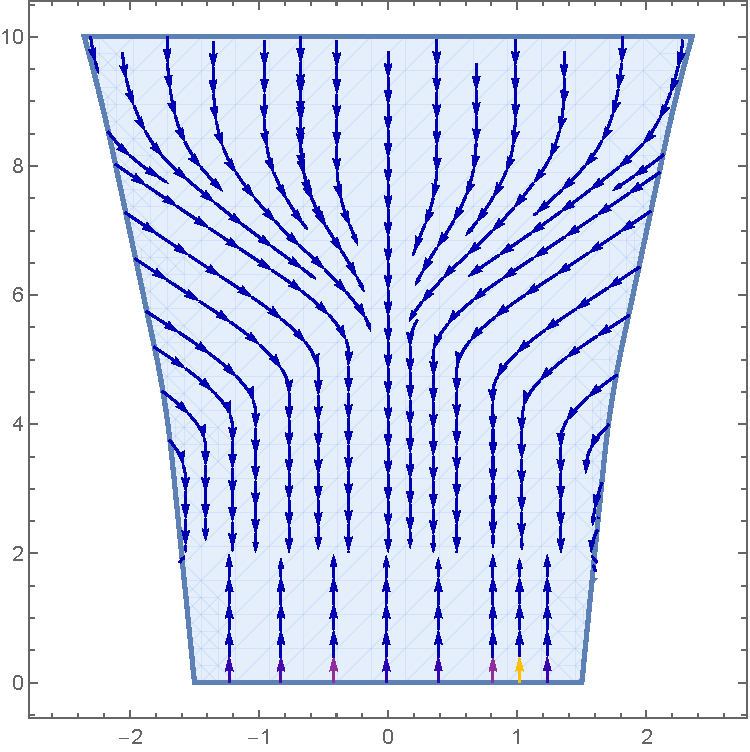
\includegraphics[width=0.4\textwidth]{figures/flow_inside.pdf}
  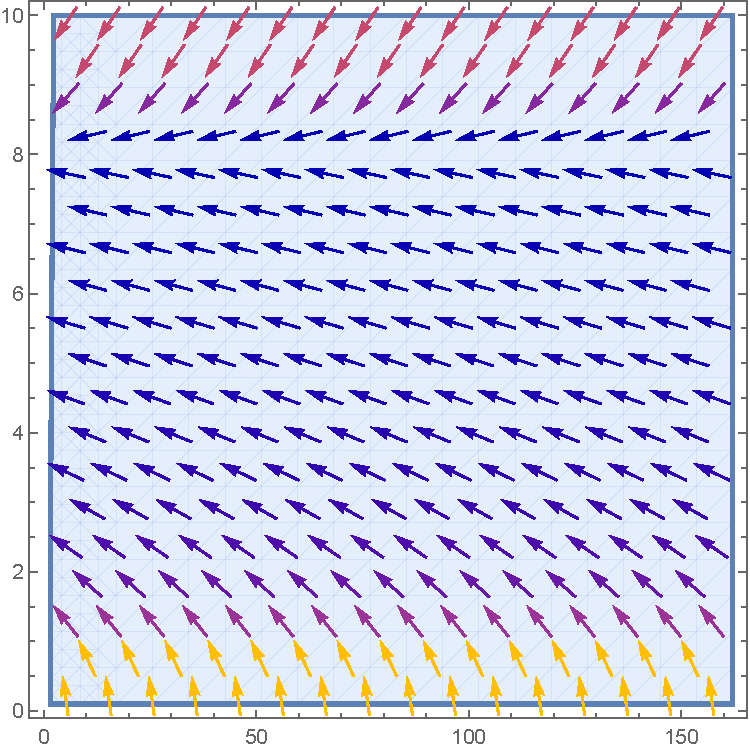
\includegraphics[width=0.4\textwidth]{figures/flow_outside.pdf}
  \caption{Left: The flow of the potential in the region where $g(x,y) \ge 10(|x|-3/2)$. Since $V$ is convex and minimal on the segment $[-\pi/2,\pi/2] \times \{2\}$, all flow lines end up on this segment. Note that the flow-lines starting from the level $y\ge 8$ end up close to the symmetry axis. Right: The vector field $-\nabla V$. The flow line originating at $(M, 0)$ is parametrized by $(M-5t, \sqrt{2t})$. We choose $M$ such that this flow line reaches the region boundary at $y=8$ after time $t=32$. Setting $t_0=50$ ensures that the flow line ends up close to the minimum. For all other flow lines on the effective boundary we have estimates that are at least as good.}
  \label{fig:flow}
\end{figure}

It is straightforward to verify that $V_B = y/2 - \log y$, which is $1/9$-strongly convex and reaches its minimum at $y=2$. Consequently, for \Cref{cond:mass}, only the mass estimate remains to be addressed, which we will cover in the following section.

Conditions 2 and 3 have been checked using Mathematica; see \Cref{fig:flow}.

\subsection{Mass estimates}

We need an upper bound for the normalization constant $Z_d = \int_{\R^2} e^{-d V(x,y)} \dd{x} \dd{y}$, which we obtain via lower bounds of the potential:
    \begin{itemize}
        \item In $[0, \pi/2] \times [0,10]$ we have $V(x,y) \ge y/2 - \log y$ with equality if $y \le 3$.
        $$J_1(s) := \int_0^s e^{-d(y/2 - \log y)} \dd{y} = 2^{d+1} \left(\frac{1}{d}\right)^{d+1} (\Gamma (d+1)-\Gamma (d+1,d s/2))$$
        \item In $[\pi/2, x_0] \times [0,10]$ we have $V(x,y) \ge f\left(\frac{2 x}{\pi}-1\right) + y/2 - \log(y)$
        $$I_1 := \int_{\pi/2}^{x_0} \exp(-d f\left(\frac{2 x}{\pi }-1\right)) \dd{x} = -\frac{\pi ^{3/2} \text{erf}\left(\frac{\sqrt{d} (\pi -2 x_0)}{\sqrt{2} \pi }\right)}{2 \sqrt{2} \sqrt{d}} \le  \frac{\pi^{3/2} c}{2 \sqrt{2} \sqrt{d}}$$
        \item In $[x_0, M] \times [0,10]$ we have $V(x,y) \ge 10(x-3/2) - \log y$
        $$I_2 :=  \int_{x_0}^{M} \exp(-d 10 (x-3/2)) \dd{x} = \frac{\left(e^{-d(10x_0-15)}-e^{-d(10 M - 15)}\right)}{10 d} \le \frac{e^{-d(10x_0-15)}}{d}$$
        and
        $$J_2 := \int_{0}^{10} \exp(-d \left(-\log (y)\right)) \dd{y} = \frac{10^{d+1}}{d+1}$$
    \end{itemize}
    Combining the above we obtain
    $$
        \mu([-\pi/2,\pi/2] \times [1,3]) \ge \frac{\pi (J_1(3)-J_1(1))}{\pi J_1(10) + I_1 J_1(10) + I_2 J_2}
    $$
    The term $I_2 J_2$ is very small;
    $$
        I_2 J_2 = \frac{10 e^{-d(10x_0-15-\log(10))}}{d^2},
    $$
    hence we can absorb it with $a$;
    $$
        \mu([-\pi/2,\pi/2] \times [1,3])  \ge \frac{1}{1  + I_1/\pi } \frac{J_1(3)-J_1(1)}{aJ_1(10)}.
    $$
    Now $\frac{J_1(3)-J_1(1)}{aJ_1(10)}$ is very close to 1, hence we can absorb it with $b$;
    $$
        \mu([-\pi/2,\pi/2] \times [1,3])  \ge \frac{1}{1  + b/\pi I_1}.
    $$
    It can be verified that $b/\pi I_1 \le \sqrt{2/d}$.

% \begin{lemma}
% For any $s \in [0,10]$ it holds that
% $$
% \int_{[-\pi/2,\pi/2] \times [0,s]} e^{-d V(x,y)} \dd{x} \dd{y} \le \pi  2^{d+1} \left(\frac{1}{d}\right)^{d+1} \left(\Gamma (d+1)-\Gamma \left(d+1,\frac{d s}{2}\right)\right).
% $$
% If \( s \le 3 \) the above holds with equality.
% \end{lemma}
% \begin{proof}
%     In \( [-\pi/2, \pi/2] \times [0,10] \) we have \( V(x,y) \ge y/2 - \log y \), with equality if \( y \le 3 \).
%     \begin{align*}
%         \int_0^s e^{-(d-1)(y/2 - \log y)} \dd{y} &= \int_0^s y^{d-1}e^{-(d-1)y/2} \dd{y} \\
%         &= \int_0^{(d-1)s/2} \left(\frac{2}{d-1}y\right)^{d-1} e^{-y} \dd{y} \\
%         &= 2^d (d-1)^{-d} \gamma(d,(d-1)s/2).
%     \end{align*}
% \end{proof}


%if $x_0 < \pi$:
%$$
%\int_{\pi/2}^{x_0} \exp(-d \, f\left(\frac{2 x}{\pi }-1\right)) \dd{x} \dd{y} = -\frac{\pi ^{3/2} \text{erf}\left(\frac{\sqrt{d} (\pi -2 s)}{\sqrt{2} \pi }\right)}{2 \sqrt{2} \sqrt{d}}
%$$
%otherwise
%$$
%\int_{\pi/2}^{\pi} \exp(-d \, f\left(\frac{2 x}{\pi }-1\right)) \dd{x} \dd{y} = \frac{\pi ^{3/2} \erf\left(\frac{\sqrt{d}}{\sqrt{2}}\right)}{2 \sqrt{2} \sqrt{d}}
%$$
%$$
%\int_{\pi}^{x_0} \exp(-d \, f\left(\frac{2 x}{\pi }-1\right)) \dd{x} \dd{y} = -\frac{\pi  e^{-\frac{2 d s}{\pi }-\frac{d}{2}} \left(e^{2 d}-e^{\frac{2 d s}{\pi }}\right)}{2 d}
%$$



\bibliographystyle{alpha}
\bibliography{references}
\newpage 

\appendix

%Here is old stuff I didn't know where to put

%\section{Meat of the proof}

\subsection{Overview}

Our goal is to show that \( \varphi^{(1)}_{V_d} \) attains its maximum in the interior of \( \Omega \), that is, \( \max_{x \in \Omega} |\varphi^{(1)}_{V_d}(x)| - \max_{x \in \partial\Omega} |\varphi^{(1)}_{V_d}(x)| > 0 \). Instead of directly finding \( \varphi^{(1)}_{V_d} \), we show that there is an approximation \( \tilde \varphi^{(1)}_{V_d} \) such that
\begin{align*}
    \text{A : } &\|\tilde\varphi^{(1)}_{V_d} - \varphi^{(1)}_{V_d}\|_{L^\infty(\mu_d)} < \delta/2 \\
    \text{B : } &\max_{x \in \Omega} |\tilde{\varphi}(x)| - \max_{x \in \partial\Omega} |\tilde{\varphi}(x)| > \delta,
\end{align*}
for some \( \delta > 0\) since then we have that
\[
    \max_{x \in \Omega} |\varphi^{(1)}_{V_d}(x)| - \max_{x \in \partial\Omega} |\varphi^{(1)}_{V_d}(x)|
    \geq \max_{x \in \Omega} |\tilde\varphi^{(1)}_{V_d}(x)| - \delta/2 - \max_{x \in \partial\Omega} |\tilde\varphi^{(1)}_{V_d}(x)| - \delta/2
    > 0.
\]

Our candidate for \( \tilde\varphi^{(1)}_{V_d} \) is \( e^{\lambda t} P_t f_0 \) for some \( f_0 \)



\remark{I the the stuff below should be reabsorbed (it mostly already is) into what I called section 2?}
\subsection{A new}

$t_{yau}$ is the time that we need to make li-yau work with dimension free constants, which is roughly 1.

\begin{enumerate}
    \item Our candidate is $f := \tilde P_{C/d}\tilde P_{t_{yau}} f_0$, where $\tilde P_t := e^{\lambda t}P_t$.
    \item By Li-Yau and the fact that $P_t$ is an $L^2$ contraction onto \( \varphi^{(1)} \), we know that \[ \|\tilde P_{t_{yau}+C/d} f_0- \varphi^{(1)}\|_\infty \le C_{yau} \|\tilde P_{C/d} f_0- \varphi^{(1)}\|_2 
    \le  C_{yau} e^{\lambda C/d} \| f_0 - \varphi^{(1)}\|_2 \]
    \item By the stable Poincare trick which works like $d^{-1/2}$-well we then have that
    $$
    \|f_0 - \varphi^{(1)}\|_2  \le \frac{\varepsilon}{\lambda^{(2)}-\lambda^{(1)}}
    $$
    with \( \varepsilon \sim d^{-1/2} \) (claim).
\end{enumerate}

\begin{equation}
    \|f-\varphi^{(1)}\|_\infty \le C_{yau} e^{\lambda C/d} \frac{\varepsilon}{\lambda^{(2)}-\lambda^{(1)}}
\end{equation}

\subsubsection{The constant}

Goal: \( C_{yau} \).

Let \( t_{yau} = t_1 + t_2 \), then \( C_{yau} = e^{\lambda t_{yau}}C_1C_2 \) where
\begin{align*}
    C_1 &\approx e^{2/t_1} (2\pi t_1)^{-1/2} \\
    C_2 &\approx \exp(\frac{5}{2t_1})\frac{t_1}{t_1 - t_2}
\end{align*}
for \( d \) large enough such that \( \Phi_{t_2 d} \) hits the line. With \( t_1 = 1.5, t_2 = 0.5 \) we obtain
\begin{align*}
    C_1 &\approx 1.25 \\
    C_2 &\approx 8
\end{align*}
together with \( \lambda \approx 2.5 \) \todo{But isn't $\lambda\approx 1$?? Also, you want to pick $t_2$ like $1/d$, and $t_1$ to minimize $t^{}$}this yields \( C_{yau} \approx 1500 \) which we can beat with \( d^{-1/2} \).

In a mathematica file i have better numbers \( C_{yau} \approx 800 \), but i still think \( d \) will be big.







 
\subsection{B new}
\begin{enumerate}
    \item  The $L^2$ norm of $\tilde P_{C/d}\tilde P_{t_{yau}} f_0$ is roughly $1$ (with respect to a probability measure). In particular, it is $\ge 1$ somewhere. Norm 1 follows from part A: \( |\|f\| - \|\varphi\|| \le \|f-\varphi\| < \frac{\varepsilon}{\lambda^{(2)}-\lambda^{(1)}} \) implies \( \|f\| \ge 1 - \frac{\varepsilon}{\lambda^{(2)}-\lambda^{(1)}} \), therefore \( f \) is at least \( 1 - \frac{\varepsilon}{\lambda^{(2)}-\lambda^{(1)}} \) somewhere.
    \item It suffices to show that it is small at the boundary.
    \item By the Liptschitz stability, the function $\tilde P_{t_{yau}} f_0$ is at most $e^{\lambda t_{yau}
    }$-lipschitz. In particular, if $g:=\tilde P_{t_{yau}} f_0$ we have the estimate
    $$
    |(P_{C/d} g)(x_0,y_0)| 
    \le |g(\Phi_C(x_0,y_0))|+e^{\lambda t_{yau}}2(C/d)^{1/2}
    \le e^{\lambda t_{yau}}(|\Phi_C(x_0,y_0)_x|+2(C/d)^{1/2})
    $$
    where the first estimate is the Gaussian estimate from the heat flow, and the second estimate is from the Liptschitz constant + the fact that we are zero at $x=0$ (antisymmetry). Let me explain the second step: \( f_0 \) is 1-Lipschitz, therefore \( g \) is \( e^{\lambda t_{yau}} \)-Lipschitz. The Lipschitz condition at \( (0, y_0) \) gives us \( |g(\Phi_C(x_0,y_0)) - g(\Phi_C(0,y_0))| \le  e^{\lambda t_{yau}}|\Phi_C(x_0,y_0) - \Phi_C(0,y_0)| \). Since \( f_0 \) is antisymmetric, \( g(\Phi_C(0,y_0)) = 0 \), hence \( |g(\Phi_C(x_0,y_0))| \le  e^{\lambda t_{yau}}|\Phi_C(x_0,y_0) - \Phi_C(0,y_0)| \). Since both flows land on the critical line, only their \( x \)-components matter. The flow line \( \Phi_C(0,y_0) \) ends up at \( (0, 2) \), therefore \( |\Phi_C(x_0,y_0) - \Phi_C(0,y_0)| = |\Phi_C(x_0,y_0)_x| \)
    \item If we flow for long enough time ($C$ big) the first term is $<1/10$, and if $d$ is big, the second term is small.
\end{enumerate}

\begin{equation*}
    \max_{x \in \Omega} |f(x)| - \max_{x \in \partial\Omega} |f(x)|
    \ge 1 -\frac{\varepsilon}{\lambda^{(2)}-\lambda^{(1)}} - e^{\lambda t_{yau}}(|\Phi_C(x_0,y_0)_x|+2(C/d)^{1/2})
\end{equation*}

% \subsection{A}

% We use ultracontractivity of \( P_t \) to reduce the problem of estimating the \( L^\infty \)-norm of \( e^{\lambda t} P_t f - \varphi^{(1)}_{V_d} \) to esimating its \( L^2 \)-norm.
% \begin{equation*}
%     \|e^{\lambda t} P_t f - \varphi \|_{L^\infty}
%     = \|e^{\lambda t} P_t f - e^{\lambda t} P_t \varphi \|_{L^\infty}
%     = e^{\lambda t} \|P_t(f-\varphi)\|_{L^\infty}
%     \le e^{\lambda t} C \|f-\varphi\|_{L^2}.
% \end{equation*}

% To apply stable Poincaré, we decompose \( f = f_{\parallel} + f_{\perp} \) into components \( f_{\parallel} \in \{\varphi^{(1)}_{V_d}\} \) and \( f_\perp \in \{\varphi^{(1)}_{V_d}\}^\perp \). We can assume that \( f \) is scaled so that \( f_\parallel = \varphi^{(1)}_{V_d} \), hence
% \[
%     \|f - \varphi^{(1)}_{V_d}\| \le \|f_\parallel - \varphi^{(1)}_{V_d}\|+ \|f_\perp\| = \|f_\perp\|.
% \]
% If we show that \( \inner{f}{\mathcal L_{V_d} f} \le (\lambda_{V_d}^{(1)} + \varepsilon)\|f\|^2 \), then using stable Poincaré we get that
% \[
%     \|e^{\lambda t} P_t f - e^{\lambda t} P_t \varphi \|_{L^\infty} \le e^{\lambda t} C \sqrt{\frac{\varepsilon}{\lambda_{V_d}^{(2)} - \lambda_{V_d}^{(1)}}} \|f\|_{L^2}
% \]

% \subsection{B}

% Show that

% \[
%     \max_{x \in \Omega} |P_tf(x)| - \max_{x \in \partial\Omega} |P_tf(x)| > e^{-\lambda t} \delta.
% \]

% We discuss how to upper bound \( P_t f(x) = \E[f(X_t)] \) in section~\ref{sec:flow}. 

% \begin{align*}
%     \max_{x \in \Omega} |P_tf(x)| - \max_{x \in \partial\Omega} |P_tf(x)|
%     &\ge \max_{x \in [-1,1] \times \{2\}} |P_tf(x)| - \max_{x \in \partial\Omega} |P_tf(x)| \\
%     &= \max_{x \in [-1,1] \times \{2\}} \E[f(X_t)|X_0=x] - \max_{x \in \partial\Omega} |\E[f(X_t)|X_0=x]| \\
%     &\ge \max_{x \in [-1,1] \times \{2\}} f(h_t(x)) - C\sqrt{2t} - \max_{x \in \partial\Omega} |f(h_t(x)) + C \sqrt{2t}| \\
%     &\ge \max_{x \in [-1,1] \times \{2\}} f(x) - C\sqrt{2t} - \max_{x \in h_t(\partial\Omega)} |f(x) + C \sqrt{2t}| \\
%     &\ge 1 - (f(x^*) + 2C \sqrt{2t})
% \end{align*}
% which is greater than \( e^{-\lambda t}\delta \) if and only if \( f(x^*) + 2C\sqrt{2t} < 1-\delta e^{-\lambda t} \).




\section{A careful computation of the Li-Yau constant.}


\remark{That's a rant for myself (jaume) but use it if it is useful}

I will assume that we have managed to prove that

\begin{proposition}
    
There exists a $t_0<64$ such that the flow by $t_0$ gets you at most $d_0<10$ far away from the center of the line.

\end{proposition}

then from here we see that
$C_1(\tau_1)^{-1} \ge \sqrt{2\pi} \tau_1^{1/2}+O(\tau).$
Eye-balling things, as long as $\tau>5$ I should have 
$C_1(\tau_1)^{-1} \ge \tau_1^{1/2}$.
which should be a good approximation as long as $\tau>10$.

We know that the $r-$axis ODE has to get to distance $\sim 8$ from the origin, and this takes us time $\sim 64/d$, and as soon as $d>64$ and $\tau>10$ should give us a negligible contribution (let's say a factor of 2 to be generous)

The total time of flight will be essentially $\tau_1$. Then for $d>10$ the total loss should be like

$2 \tau_1^{-1/2}e^{\tau_1 x_0+\tau_2} \le 2^{3/2} e x_0^{1/2} (2\tau_1x_0e^{-2 \tau_1 x_0})^{-1/2}$.

Optimizing over $\tau_1$ amounts to finding the largest value of $xe^{-x}$, which is $1/e$ taken at $\tau = \frac{1}{2 x_0}$. In other words, we get that the Li-Yau constant will be like $(2e)^{3/2} x_0^{1/2}$ and setting $x_0=10$, we get a li-yau constant of $40$ (but more like $14\cdot e^{64/d}$ in case $d$ gets big and it's useful)

Now the constant $C_{SP}$ will be like 

\subsection{A much better eigenfunction estimate than cosine}

If we were able to give a good Lip constant to the eigenfunction itself we would be a lot more efficient. 



\includepdf[pages=-]{declaration}


\end{document}
